\documentclass{article}
\usepackage[a4paper, portrait, margin=2cm]{geometry}
\usepackage[hungarian]{babel}
\usepackage{amsfonts}
\usepackage{amsmath}
\usepackage{enumitem}
\usepackage[numbered]{bookmark}
\usepackage{hyperref}
\usepackage[parfill]{parskip}
\usepackage[table,xcdraw]{xcolor}
\usepackage{soul}
\usepackage{tikz}
\usepackage{float}
\usepackage{algorithm}
\usepackage{algorithmic}
\usepackage{pgfplots}
\usepackage{MnSymbol}
\pgfplotsset{compat=1.11}
\usetikzlibrary{positioning, arrows.meta, calc, shapes.geometric, snakes}

\makeatletter
\renewcommand{\Hy@numberline}[1]{#1. }
\makeatother

\newcommand{\angledarrow}[1]{
    \begin{tikzpicture}[scale=0.4]
    \draw[->, rotate=#1] (0, 0) -- (1, 0);
    \end{tikzpicture}
}

\begin{document}
\section{gyakorlat (2025. szeptember 10.)}
\subsection{Stabil párosítás}
\subsubsection*{Naiv algoritmus (nem feltétlen termináló)}
Könyv: \url{../konyv.pdf#page=105}

\begin{tabular}{l l}
    $f_1 \rightarrow (l_2, l_1, l_3)$ & $l_1 \rightarrow (f_1, f_3, f_2)$ \\
    $f_2 \rightarrow \text{tetszőleges, pl. } (l_1, l_2, l_3)$ & $l_2 \rightarrow (f_3, f_1, f_2)$ \\
    $f_3 \rightarrow (l_1, l_2, l_3)$ & $l_3 \rightarrow \text{tetszőleges, pl. } (f_1, f_2, f_3)$ \\
\end{tabular}

\textbf{Algoritmus}
\begin{enumerate}
    \item Keressünk instabilitást a párosításban: egy fiúnak jobban tetszik egy másik lány ÉS a lánynak jobban tetszik egy másik fiú.
    \item Az (egyik) instabilitásbeli \ul{négyest} felcseréljük.
\end{enumerate}

\setulcolor{red}
\textbf{Kezdeti párosítás:} $M_0=\left\{\text{\ul{$(f_1, l_1)$}}, \text{\ul{$(f_2, l_2)$}}, (f_3, l_3)\right\}$, ez nem stabil.\\
\textbf{Instabilitás:} $\left[f_3-l_2\right]$ és \ul{$\left[f_1-l_2\right]$} (több van, ezért \ul{választunk} egyet)

\setulcolor{blue}
$M_1=\left\{\text{\ul{$(f_1, l_2)$}}, (f_2, l_1), \text{\ul{$(f_3, l_3)$}}\right\}$\\
\textbf{Instabilitás:} \ul{$\left[f_3-l_2\right]$} és $\left[f_3-l_1\right]$

\setulcolor{green}
$M_2=\left\{(f_1, l_3), \text{\ul{$(f_2, l_1)$}}, \text{\ul{$(f_3, l_2)$}}\right\}$\\
\textbf{Instabilitás:} $\left[f_1-l_1\right]$ és \ul{$\left[f_3-l_1\right]$}

\setulcolor{orange}
$M_3=\left\{\text{\ul{$(f_1, l_3)$}}, \text{\ul{$(f_2, l_2)$}}, (f_3, l_1)\right\}$\\
\textbf{Instabilitás:} $\left[f_1-l_2\right]$ és \ul{$\left[f_1-l_1\right]$}

$M_4=\left\{(f_1, l_1), (f_2, l_2), (f_3, l_3)\right\} = M_0$\\
Végtelen ciklus: $M_0, M_1, M_2, M_3, M_4=M_0, M_1, M_2, \cdots$


\subsubsection*{Gale-Shapley algoritmus}
\sethlcolor{orange}
\hl{(zh. feladat)}

\setstcolor{red}
\begin{tabular}{l l}
    $f_1 \rightarrow (\text{\st{$l_3$}}, \text{\st{$l_2$}}, l_5, l_1, l_4)$ & $l_1 \rightarrow (f_3, f_5, f_2, f_1, f_4)$ \\
    $f_2 \rightarrow (\text{\st{$l_1$}}, l_2, l_5, l_3, l_4)$ & $l_2 \rightarrow (f_5, f_2, f_1, f_4, f_3)$ \\
    $f_3 \rightarrow (l_4, l_3, l_2, l_1, l_5)$ & $l_3 \rightarrow (f_4, f_3, f_5, f_1, f_2)$ \\
    $f_4 \rightarrow (\text{\st{$l_1$}}, l_3, l_4, l_2, l_5)$ & $l_4 \rightarrow (f_1, f_2, f_3, f_4, f_5)$ \\
    $f_5 \rightarrow (l_1, l_2, l_4, l_5, l_3)$ & $l_5 \rightarrow (f_2, f_3, f_4, f_1, f_5)$ \\
\end{tabular}

\begin{tabular}{c|c|c|c|c|c|}
    & $l_1$ & $l_2$ & $l_3$ & $l_4$ & $l_5$ \\
    \hline
    1. & $f_2$, $f_4$, \fbox{$f_5$} &  & $f_1$ & $f_3$ &  \\
    2. & $f_5$ & $f_2$ & $f_1$, \fbox{$f_4$} & $f_3$ &  \\
    3. & $f_5$ & \fbox{$f_2$}, $f_1$ & $f_4$ & $f_3$ &  \\
    4. & $f_5$ & $f_2$ & $f_4$ & $f_3$ & $f_1$ \\
\end{tabular}

\textbf{Észrevétel 1:} mindig van egy lány, akinél csak az utolsó napon jelenik meg egy szerenádozó.
Ezt a lányt senki sem húzza ki a preferencialistájáról.\\
\textbf{Észrevétel 2:} a többi lányt legalább 1 fiú nem húzza ki.\\
Kihúzások száma: $n^2-n-(n-1)=(n-1)^2+1$

\textbf{Hány nap alatt fejeződik be biztosan?} Előadás: $n^2+1$ korlát (minden nap legalább 1 lányt kihúznak).\\
\textbf{Észrevétel 1:} $n^2+1-n$\\
\textbf{Észrevétel 2:} $n^2+1-n-(n-1)$ (a végén n-1 mert az első észrevételbeli lányt nem számoljuk még egyszer)\\
\textbf{Összesen:} $n^2+1-n-(n-1)=(n^2-2n+1)+1=(n-1)^2+1$


\textbf{Maximum hány stabil párosítás lehetséges n fiú és n lány között?} Az összes teljes párosítás száma: $n!$.
Gale-Shapley algoritmus: mindig van legalább 1.\\
\textbf{HF.} Ha minden lánynak ugyanaz a preferencialistája, akkor csak 1 létezik.
Észrevétel: néha 1-nél több van.

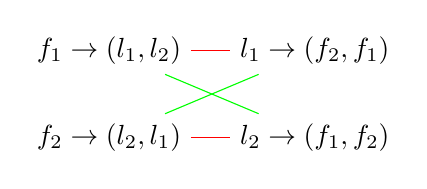
\begin{tikzpicture}
\node(f1){$f_1 \rightarrow (l_1, l_2)$};
\node(l1)[right = 0.5cm of f1]{$l_1 \rightarrow (f_2, f_1)$};
\node(f2)[below = 0.5cm of f1]{$f_2 \rightarrow (l_2, l_1)$};
\node(l2)[below = 0.5cm of l1]{$l_2 \rightarrow (f_1, f_2)$};
\draw[red] (f1) -- (l1);
\draw[red] (f2) -- (l2);
\draw[green] (f1) -- (l2);
\draw[green] (f2) -- (l1);
\end{tikzpicture}

{\color{red} Stabil párosítás:} minden \textbf{fiú} a preferencialistájának elsőjét kapja.\\
{\color{green} Stabil párosítás:} minden \textbf{lány} a preferencialistájának elsőjét kapja.

\textbf{Meglepetés:}
$2n$ fiú és $2n$ lány van, akár $2^n$ párosítás is lehetséges.\\
\begin{tabular}{l l}
    $f_1 \rightarrow (l_1, l_2, \cdots)$ & $l_1 \rightarrow (\cdots, f_1)$ \\
    $f_2 \rightarrow (l_2, l_1, \cdots)$ & $l_2 \rightarrow (\cdots, f_2)$ \\
    $f_3 \rightarrow (l_3, l_4, \cdots)$ & $l_3 \rightarrow (\cdots, f_3)$ \\
    $f_4 \rightarrow (l_4, l_3, \cdots)$ & $l_4 \rightarrow (\cdots, f_4)$ \\
    $f_{2i-1} \rightarrow (l_{2i-1}, l_{2i}, \cdots)$ & $l_1 \rightarrow (\cdots, f_{2i-1})$ \\
    $f_{2i} \rightarrow (l_{2i}, l_{2i-1}, \cdots)$ & $l_1 \rightarrow (\cdots, f_{2i})$ \\
    \vdots & \vdots \\
    $f_{2n-1} \rightarrow (l_{2n-1}, l_{2n}, \cdots)$ & $l_1 \rightarrow (\cdots, f_{2n-1})$ \\
    $f_{2n} \rightarrow (l_{2n}, l_{2n-1}, \cdots)$ & $l_1 \rightarrow (\cdots, f_{2n})$ \\
\end{tabular}

A sok-sok stabil párosítás:

\raisebox{-.4\height}{
\fbox{
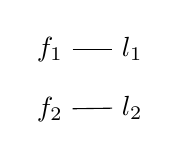
\begin{tikzpicture}
\node(f1){$f_1$};
\node(l1)[right = 0.5cm of f1]{$l_1$};
\node(f2)[below = 0.2cm of f1]{$f_2$};
\node(l2)[below = 0.2cm of l1]{$l_2$};
\draw (f1) -- (l1);
\draw (f2) -- (l2);
\end{tikzpicture}
}
}
vagy
\raisebox{-.4\height}{
\fbox{
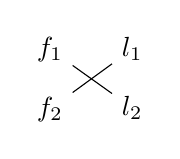
\begin{tikzpicture}
\node(f1){$f_1$};
\node(l1)[right = 0.5cm of f1]{$l_1$};
\node(f2)[below = 0.2cm of f1]{$f_2$};
\node(l2)[below = 0.2cm of l1]{$l_2$};
\draw (f1) -- (l2);
\draw (f2) -- (l1);
\end{tikzpicture}
}
}

\raisebox{-.4\height}{
\fbox{
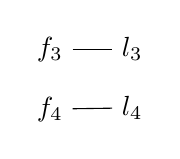
\begin{tikzpicture}
\node(f3){$f_3$};
\node(l3)[right = 0.5cm of f3]{$l_3$};
\node(f4)[below = 0.2cm of f3]{$f_4$};
\node(l4)[below = 0.2cm of l3]{$l_4$};
\draw (f3) -- (l3);
\draw (f4) -- (l4);
\end{tikzpicture}
}
}
vagy
\raisebox{-.4\height}{
\fbox{
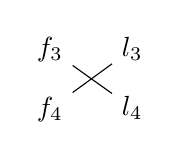
\begin{tikzpicture}
\node(f3){$f_3$};
\node(l3)[right = 0.5cm of f3]{$l_3$};
\node(f4)[below = 0.2cm of f3]{$f_4$};
\node(l4)[below = 0.2cm of l3]{$l_4$};
\draw (f3) -- (l4);
\draw (f4) -- (l3);
\end{tikzpicture}
}
}

Minden sorból választunk egyet: $2^n$ lehetőség.\\
\textbf{HF. } az összes így kapott párosítás stabil (nincs instabilitás).

\textbf{Miért lesz ez mind stabil párosítás?}

Ha a felső kockát választottuk, akkor $f_1$ párja a preferencialistáján az első lány, így $f_1$ nem lehet instabilitás fiú tagja.

Ha az alsó kockát választottuk, akkor $f_1$ párja a preferencialistáján a második lány, így $f_1$ csak az $l_1$ lánnyal lehet instabilitásban.
Azonban $f_1$ utolsó $l_1$ preferencialistáján, így akárki is $l_1$ párja, ő jobban tetszik $l_1$-nek, mint $f_1$.
Így $f_1$ most sem lehet instabilitás fiú tagja.

Ez a gondolatmenet minden fiúra alkalmazható, így mind a $2^n$ párosítás stabil.

\clearpage
\section {gyakorlat (2025. szeptember 17.)}
\textbf{Miért lesz ez mind stabil párosítás?}

Ha a felső kockát választottuk, akkor $f_1$ párja a preferencialistáján az első lány, így $f_1$ nem lehet instabilitás fiú tagja.

Ha az alsó kockát választottuk, akkor $f_1$ párja a preferencialistáján a második lány, így $f_1$ csak az $l_1$ lánnyal lehet instabilitásban.
Azonban $f_1$ utolsó $l_1$ preferencialistáján, így akárki is $l_1$ párja, ő jobban tetszik $l_1$-nek, mint $f_1$.
Így $f_1$ most sem lehet instabilitás fiú tagja.

Ez a gondolatmenet minden fiúra alkalmazható, így mind a $2^n$ párosítás stabil.

\subsubsection*{Stabil szobatárs probléma}
Nem feltétlenül létezik stabil párosítás.

$A \rightarrow (B, C, D)$\\
$B \rightarrow (C, A, D)$\\
$C \rightarrow (A, B, D)$\\
$D \rightarrow mindegy$\\

Három teljes párosítás létezik, A párja egyértelműen meghatározza a párosítást.
\begin{enumerate}
    \item $(A, B), (C, D) \rightarrow$ instabilitás: B és C
    \item $(A, C), (B, D) \rightarrow$ instabilitás: A és B
    \item $(A, D), (B, C) \rightarrow$ instabilitás: A és C
\end{enumerate}
Így itt nincs stabil párosítás.

\subsubsection*{Feladat}
Legyen $M_1$ és $M_2$ két különböző stabil házasítás (visszatértünk az eredeti fiú-lány feladathoz).
Minden fiúhoz rendeljük hozzá az $M_1$ és $M_2$-beli párja közül a neki jobban tetszőt.
Mutassuk meg, hogy így teljes párosítást kapunk (nem triviális) ami ráadásul stabil.

\textbf{Teljes párosítás}

Indirekt tegyük fel, hogy ez nem teljesül, következésképpen vannak olyan $f'$ és $f''$ különböző fiúk, hogy:

$M_1:$
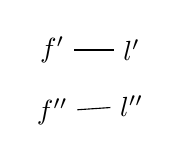
\begin{tikzpicture}
\node(f'){$f'$};
\node(l')[right = 0.5cm of f']{$l'$};
\node(f'')[below = 0.2cm of f']{$f''$};
\node(l'')[below = 0.2cm of l']{$l''$};
\draw (f') -- (l');
\draw (f'') -- (l'');
\end{tikzpicture}
és $M_2:$
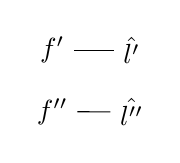
\begin{tikzpicture}
\node(f'){$f'$};
\node(l')[right = 0.5cm of f']{$\hat{l'}$};
\node(f'')[below = 0.2cm of f']{$f''$};
\node(l'')[below = 0.2cm of l']{$\hat{l''}$};
\draw (f') -- (l');
\draw (f'') -- (l'');
\end{tikzpicture}

és $JobbanTetszik_{f'}(l',\hat{l}') = JobbanTetszik_{f''}(l'',\hat{l}'')$
Az általánosság megszorítása nélkül feltehetjük, hogy $JobbanTetszik_{f'}(l', l'') = l'$ és $JobbanTetszik_{f''}(l', \hat{l}'') = l''$.

Ha ez nem elég meggyőző: négy eset van:
\begin{enumerate}
    \item $JT_{f'}(l', \hat{l}') = l'$ és $JT_{f''}(l'', \hat{l}'') = l''$
    \item $JT_{f'}(l', \hat{l}') = l'$ és $JT_{f''}(l'', \hat{l}'') = \hat{l}''$
    \item $JT_{f'}(l', \hat{l}') = \hat{l}'$ és $JT_{f''}(l'', \hat{l}'') = l''$
    \item $JT_{f'}(l', \hat{l}') = \hat{l}'$ és $JT_{f''}(l'', \hat{l}'') = \hat{l}'' \rightarrow$ nem lehet 
\end{enumerate}

\textbf{HF. }
Keressünk instabilitást $M_1$-ben vagy $M_2$-ben.

\textbf{Feladat.}
Hosszú Gale-Shapley algoritmus futás.
Először adott 5 fiú - 5 lány.

\begin{tabular}{c|c|c|c|c|c|}
    & $l_1$ & $l_2$ & $l_3$ & $l_4$ & $l_5$ \\
    \hline
    1. & \fbox{$f_1$}, $f_5$ & $f_2$ & $f_3$ & $f_4$ &  \\
    2. & $f_1$ & \fbox{$f_2$}, $f_5$ & $f_3$ & $f_4$ &  \\
    3. & $f_1$ & $f_2$ & \fbox{$f_3$}, $f_5$ & $f_4$ &  \\
    4. & $f_1$ & $f_2$ & $f_3$ & $f_4$, \fbox{$f_5$} &  \\
    5. & \fbox{$f_1$}, $f_4$ & $f_2$ & $f_3$ & $f_5$ &  \\
    6. & $f_1$ & \fbox{$f_2$}, $f_4$ & $f_3$ & $f_5$ &  \\
    7. & $f_1$ & $f_2$ & $f_3$, \fbox{$f_4$} & $f_5$ &  \\
    8. & $f_1$ & $f_2$ & $f_4$ & \fbox{$f_5$}, $f_3$ &  \\
    9. & \fbox{$f_1$}, $f_3$ & $f_2$ & $f_4$ & $f_5$ &  \\
    10. & $f_1$ & $f_2$, \fbox{$f_3$} & $f_4$ & $f_5$ &  \\
    11. & $f_1$ & $f_3$ & \fbox{$f_4$}, $f_2$ & $f_5$ &  \\
    12. & $f_1$ & $f_3$ & $f_4$ & \fbox{$f_5$}, $f_2$ &  \\
    13. & $f_1$, \fbox{$f_2$} & $f_3$ & $f_4$ & $f_5$ &  \\
    14. & $f_2$ & \fbox{$f_3$}, $f_1$ & $f_4$ & $f_5$ &  \\
    15. & $f_2$ & $f_3$ & \fbox{$f_4$}, $f_1$ & $f_5$ &  \\
    16. & $f_2$ & $f_3$ & $f_4$ & \fbox{$f_5$}, $f_1$ &  \\
    17. & $f_2$ & $f_3$ & $f_4$ & $f_5$ & $f_1$ \\
\end{tabular}

Ez általánosítható bármely számú fiúra és lányra $\rightarrow (n-1)^2 + 1$ nap.

\textbf{HF.} "Konstruáljuk meg" a preferencialistákat.\\
\textbf{HF.} Nem létezik olyan teljes párosítás (stabil vagy nem stabil), amelyben minden fiúnak szigorúan jobban tetszik a párja, mint a Gale-Shapley algoritmus által szolgáltatott párja.

\clearpage
\section {gyakorlat (2025. szeptember 24.)}
\textbf{Állítás (pareto optimalitás):}
Jelölje $M$ a Gale-Shapley algoritmus által szolgáltatott (fiú-optimális) párosítást.
Ekkor nem létezik olyan $M'$ teljes párosítás (nem stabil sem), ahol minden fiú jobban jár mint $M$-ben.
(Olyat valószínűleg tudunk mutatni, amiben valamelyik fiú jobban jár mint $M$-ben, mivel a Gale-Shapley algoritmus esetén lehet olyan fiú aki nem a listájáról az első lányt kapta.
Ha ez a fiú megkapja a listájának első lányát (és a többi fiú is valamilyen módon kap egy új párt), akkor máris mutattunk egy ilyen párosítást.)

\textbf{Bizonyítás:}
Indirekt tegyük fel, hogy létezik olyan $M'$ teljes párosítás, ahol minden fiú jobban jár, mint $M$-nél.
Nézzük az M-et előállító Gale-Shapley algoritmus lefutását.
Ekkor van olyan $l$ lány, akinek csak az utolsó napon jelenik meg az ablaka alatt szerenádozó, aki végül a párja lesz.
Legyen ez a fiú $f$.
Most $f$ $M'$-beli $l'$ párja jobban tetszik $f$-nek, mint $l$ (spec. $l' \neq l$).
Jelölje $l$ $M$-beli párját $f'$.
Ismét, $f'$ $M'$-beli $l$ párja jobban tetszik $f'$-nek, mint az $M$-beli párja.

Igen ám, de ekkor $f'$ az utolsó nap előtt szerenádozott $l$-nél és kosarat kapott, ellentmondva annak, hogy $l$-nél csak az utolsó nap szerenádozik valaki.

\subsection*{Megoldandó probléma}
$T(n) = a T\left(\frac{n}{b}\right) + f(n)$ alakú rekurziók.

\textbf{Összefésüléses rendezés}\\
$T(n) = 2 T\left(\frac{n}{2}\right) + n \rightarrow T(n) = \Theta(n \log n)$

\textbf{Maximális növekedés}\\
Adott pozitív számoknak egy $A[1:n]$ tömbje.
Keressünk olyan $1 \leq i \leq j \leq n$ indexeket, hogy $A[j] - A[i]$ maximális.

\subsection*{Oszd meg és uralkodj algoritmusok}
Oszd meg és uralkodj algoritmust tervezünk (van más, hatékony módszer is).
\begin{enumerate}
    \item Bontsuk a feladatot két feleakkora méretű feladatra:
    \begin{itemize}
        \item $A[1: \frac{n}{2}]$-ben hol van a maximális növekedés
        \item $A[\frac{n}{2} + 1: n]$-ben hol van a maximális növekedés
    \end{itemize}
    \item Rekurzívan megoldjuk a részfeladatokat:
    \begin{itemize}
        \item $A[1: \frac{n}{2}] \rightarrow 1 \leq i' \leq j' \leq \frac{n}{2}$
        \item $A[\frac{n}{2} + 1: n] \rightarrow \frac{n}{2} + 1 \leq i'' \leq j'' \leq n$
    \end{itemize}
    Egyelemű tömbökre direkt megoldás: a két index megegyezik az elem indexével.
    \item A maximális növekedést adó $i$ és $j$ meghatározása. Három eset van:
    \begin{enumerate}
        \item $A[1: \frac{n}{2}]$-ben (az első felében) van a maximális növekedés $\rightarrow i = i' \text{ és } j = j'$
        \item $A[\frac{n}{2} + 1: n]$-ben (a második felében) van a maximális növekedés $\rightarrow i = i'' \text{ és } j = j''$
        \item $1 \leq i \leq \frac{n}{2} < j \leq n$ (az egyik az első, a másik a második felében). Ekkor $i$-t célszerű úgy választani, hogy $A[i]$ az $A[1: \frac{n}{2}]$ legkisebb értéke, $j$-t pedig úgy, hogy $A[j]$ az $A[\frac{n}{2} + 1: n]$ legnagyobb értéke.
    \end{enumerate}
\end{enumerate}

Nem tudjuk előre, hogy (a), (b) és (c) közül melyik adja az optimumot, ezért mindet megvizsgáljuk és a legkedvezőbbet választjuk.

\subsubsection*{Költség}
$T(n) = \underbrace{2 T (\frac{n}{2})}_{\text{két rekurzív hívás}} + \underbrace{\Theta(n)}_{\text{\parbox{4.1cm}{\centering min $A[1:\frac{n}{2}]$-ben \\ max $A[\frac{n}{2}+1: n]$-ben \\ (a), (b), (c) "közül a legnagyobb"}}}$

Ez egy összefésüléses rendezés rekurzió $\rightarrow T(n) = \Theta(n \log n)$

\clearpage
\textbf{Van hatékonyabb?} Nem meglepő módon igen:

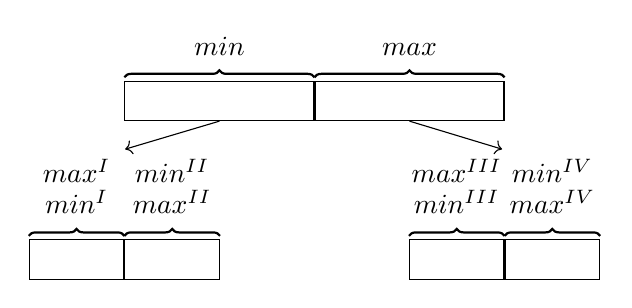
\begin{tikzpicture}[
    squarenodebig/.style={rectangle, draw=black, minimum width=2.4cm, minimum height=0.5cm},
    squarenodesmall/.style={rectangle, draw=black, minimum width=1.2cm, minimum height=0.5cm}
]
\node[squarenodebig](arr_1_1){};
\node[squarenodebig](arr_1_2)[right = 0cm of arr_1_1]{};
\node[squarenodesmall](arr_2_1)[below left = 1.5cm and 0cm of arr_1_1]{};
\node[squarenodesmall](arr_2_2)[right = 0cm of arr_2_1]{};
\node[squarenodesmall](arr_2_4)[below right = 1.5cm and 0cm of arr_1_2]{};
\node[squarenodesmall](arr_2_3)[left = 0cm of arr_2_4]{};

\draw[thick, decoration={brace, raise=0.3cm}, decorate] (arr_1_1.west) -- (arr_1_1.east);
\draw[thick, decoration={brace, raise=0.3cm}, decorate] (arr_1_2.west) -- (arr_1_2.east);
\draw[thick, decoration={brace, raise=0.3cm}, decorate] (arr_2_1.west) -- (arr_2_1.east);
\draw[thick, decoration={brace, raise=0.3cm}, decorate] (arr_2_2.west) -- (arr_2_2.east);
\draw[thick, decoration={brace, raise=0.3cm}, decorate] (arr_2_3.west) -- (arr_2_3.east);
\draw[thick, decoration={brace, raise=0.3cm}, decorate] (arr_2_4.west) -- (arr_2_4.east);

\node[above = 0.2cm of arr_1_1]{$min$};
\node[above = 0.2cm of arr_1_2]{$max$};
\node[above = 0.2cm of arr_2_1]{$min^{I}$};
\node[above = 0.6cm of arr_2_1]{$max^{I}$};
\node(min2)[above = 0.6cm of arr_2_2]{$min^{II}$};
\node[above = 0.2cm of arr_2_2]{$max^{II}$};
\node[above = 0.2cm of arr_2_3]{$min^{III}$};
\node[above = 0.6cm of arr_2_3]{$max^{III}$};
\node(min4)[above = 0.6cm of arr_2_4]{$min^{IV}$};
\node[above = 0.2cm of arr_2_4]{$max^{IV}$};

\draw[->] (arr_1_1.south) -- (min2.north west);
\draw[->] (arr_1_2.south) -- (min4.north west);
\end{tikzpicture}

A rekurzív hívásokba süllyesztve a min és max kiválasztást $\Theta(n)$ $\Theta(1)$-re csökken a rekurzióban.

Zárt formula erre: $T(n) = 2T (\frac{n}{2}) + 1$\\
\textbf{HF. } direkt számolás (önmagába helyettesítés)

Még egy érdekes dolog:\\
$T(n) = T(\frac{n}{2}) + 1 \rightarrow T(n) = \Theta(\log n)$\\
$T(n) = T(\frac{n}{2}) + n \rightarrow T(n) = \Theta(n)$

\subsection{Mester-tétel}
Könyv: \url{../konyv.pdf#page=10}\\
$f(n) \leftrightarrow n^{\log_b a}$

\begin{enumerate}
    \item
    \begin{itemize}
        \item $T(n) = aT\left(\frac{n}{b}\right) + f(n) = 9T\left(\frac{n}{3}\right) + n$
        \item $n^{\log_b a} = n^{\log_3 9} = n^2$ polinomiálisan nagyobb, mint $f(n)$
        \item $[f(n) = n = O(n^{2-\mathcal{E}})$, például $\mathcal{E}=\frac{1}{2}$ esetén$]$
        \item Mester tétel első eset $\rightarrow T(n) = \Theta(n^{log_b a}) = \Theta(n^2)$
    \end{itemize}
    \item
    \begin{itemize}
        \item $T(n) = T\left(\frac{2n}{3}\right) + 1$ ($a=1$, $b=\frac{3}{2}$, $f(n) = 1$)
        \item $n^{log_b a} = n^{log_{\frac{3}{2}} 1} = n^0 = 1$ aszimptotikusan megegyezik $f(n)$-nel.
        \item $[f(n) = 1 = \Theta(n^0) = \Theta(1)]$
        \item Mester tétel második eset $\rightarrow T(n) = \Theta(n^{\log_b a} \log n) = \Theta(\log n)$ 
    \end{itemize}
        \item
    \begin{itemize}
        \item $T(n) = 3T\left(\frac{n}{4}\right) + n \log n$ ($a=3$, $b=4$, $f(n) = n \log n$)
        \item $n^{log_b a} = n^{log_4 3} \approx n^{0,793}$ ($\log_4 3 < log_4 4 = 1$)
        \item $f(n)$ polinomiálisan nagyobb, mint $n^{0,793}$
        \item $f(n) = n \log n = \Omega(n^{0,793 + \mathcal{E}})$ pl. $\mathcal{E}=0,1$ esetén
        \item A Mester tétel harmadik esetének néz ki, de ahhoz hogy tényleg az legyen, még egy dolgot ellenőrizni kell:
        \begin{itemize}[label=$\diamond$]
            \item a $f\left(\frac{n}{b}\right) \leq c f(n)$ alkalmas $c < 1$ konstanssal
            \item $3 f\left(\frac{n}{4}\right) = 3 \left(\frac{n}{4} \log \frac{n}{4}\right) = \frac{3}{4} n \log \frac{n}{4} \leq \frac{3}{4} n \log n$
            \item $c = \frac{3}{4}$ megfelelő
            \item Így tényleg mester tétel harmadik eset $\rightarrow T(n) = \Theta(f(n)) = \Theta(n \log n)$
        \end{itemize}
    \end{itemize}
\end{enumerate}

\textbf{HF. } mindenféle ilyen rekurziók:
\begin{itemize}
    \item $T(n) = 2T\left(\frac{n}{2}\right) + n^3$
    \item $T(n) = 2T\left(\frac{n}{2}\right) + n^2$
    \item $T(n) = 2T\left(\frac{n}{2}\right) + n \log n$
\end{itemize}

\clearpage
\section{gyakorlat (2025. október 1.)}
\textbf{"Oszd meg és uralkodj"}
\begin{enumerate}
    \item részproblémákra bontjuk
    \item a részproblémákat megoldjuk
    \item ezek eredményéből kiszámoljuk a végeredményt
\end{enumerate}

\subsubsection*{Inverziószámok keresése/számlálása}
Legyen $A[1..n]$ egy tömb egyedi számokkal. Az $(i, j)$ indexpár inverzió, ha $1 \leq i < j \leq n$ és $A[i] > A[j]$.
Számoljuk meg, hány inverzió van a tömbben.

\textbf{Naiv módszer:}\\
Minden indexpárt ellenőrzünk: $O(n^2)$.

\textbf{Oszd meg és uralkodj:}\\
(könyv: \url{../konyv.pdf#page=8})
\begin{enumerate}
    \item Részproblémákra bontjuk: külön keressük az inverziókat $A[1:\frac{n}{2}]$ és $A[\frac{n}{2}+1:n]$-ben
    \item A részproblémák megoldása (rekurzívan): ha a részprobléma 1 elemű, akkor nincs inverzió, adjunk vissza 0-t
    \item Válaszok egyesítése: keressük az összes inverziót.
    \begin{enumerate}
        \item $1 \leq i < j \leq \frac{n}{2} \rightarrow A[1: \frac{n}{2}]$ részprobléma
        \item $\frac{n}{2} + 1 \leq i < j \leq n \rightarrow A[\frac{n}{2} + 1: n]$ részprobléma
        \item $1 \leq i \leq \frac{n}{2} < j \leq n \rightarrow \; ?$
    \end{enumerate}
\end{enumerate}

Ötlet: rendezzünk menet közben (merge sort).
Ha rendezett a két résztömb, könnyebb a (c) esetet ellenőrizni.
Két eset van:
\begin{itemize}
    \item $A[i] < A [j] \rightarrow$ nincs inverzió. Mivel rendezett a tömb, ezért minden ($j \leq k \leq n$) $k$ index se lesz inverzió.
    \item $A[i] > A[j] \rightarrow$ inverzió. Mivel rendezettek a tömbök, ezért minden ($i \leq l \leq \frac{n}{2}$) $l$ index is inverzió lesz j-vel.
\end{itemize}

\textbf{Végeredmény:} a két részprobléma megoldásai + a köztük végzett ellenőrzés eredménye.
Futási idő: $\mathcal{O}(n \cdot \log n)$ mint a merge sort.

\subsubsection*{Többségi elem keresése}
Egy elem többségi elem egy $A[1:n]$ tömbben, ha $\frac{n}{2}$-nél többször fordul elő benne (pl. minimum 6/10, minimum 4/7, stb.).
Ha van többségi elem egy tömbben, akkor biztosan egy van.
Keressük meg a többségi elemet, amennyiben van ilyen.

\textbf{Naiv módszer:}\\
Minden elemet megszámolunk: $O(n^2)$.

\textbf{Oszd meg és uralkodj:}
\begin{enumerate}
    \item Részproblémák:
    \begin{itemize}
        \item Ötlet: ha $x$ többségi elem $A[1:n]$ tömbben, akkor (mivel $\frac{n}{2}$-nél többször fordul elő) többségi elem lesz $A[1:\frac{n}{2}]$-ben vagy $A[\frac{n}{2}+1:n]$-ben.
        \item Szóval a részproblémák: vegyük a tömb egyik ($A[1:\frac{n}{2}]$) és másik ($A[\frac{n}{2}+1:n]$) felét. 
    \end{itemize}
    \item Részproblémák megoldása rekurzívan:
    \begin{itemize}
        \item Ha 1 elemű a tömb, akkor az az elem a többségi elem.
        \item $A[1:\frac{n}{2}] \rightarrow m'$, $A[\frac{n}{2}+1:n] \rightarrow m''$ ($m'$ és $m''$ lehet üres is (ha nincs többségi elem az adott résztömbben))
        \item $m'$ és $m''$ közül valamelyik az egész tömb többségi eleme is lesz.
    \end{itemize}
    \item Számoljuk meg az előfordulásokat, hogy $m'$ és $m''$ hányszor szerepel $A[1:n]$-ben.
    \begin{itemize}
        \item Ha $m'$ többször fordul elő, mint $m''$, akkor $m'$ lesz a többségi elem.
        \item Ha $m''$ többször fordul elő, mint $m'$, akkor $m''$ lesz a többségi elem.
        \item Ha $m'$ és $m''$ ugyanannyiszor fordul elő, akkor nincs többségi elem.
    \end{itemize}
\end{enumerate}

\textbf{Futási idő:} $\mathcal{O}(n \log n)$

\textbf{Tudunk-e erre a problémára hatékonyabb (lineáris) algoritmust?}
Igen, de nem oszd meg és uralkodj.

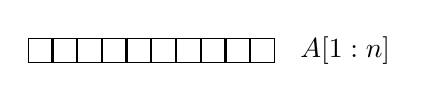
\begin{tikzpicture}[
    squarenode/.style={rectangle, draw=black, minimum width=0.3cm, minimum height=0.3cm},
]
\node[squarenode](a1){};
\node[squarenode](a2)[right = 0cm of a1]{};
\node[squarenode](a3)[right = 0cm of a2]{};
\node[squarenode](a4)[right = 0cm of a3]{};
\node[squarenode](a5)[right = 0cm of a4]{};
\node[squarenode](a6)[right = 0cm of a5]{};
\node[squarenode](a7)[right = 0cm of a6]{};
\node[squarenode](a8)[right = 0cm of a7]{};
\node[squarenode](a9)[right = 0cm of a8]{};
\node[squarenode](a10)[right = 0cm of a9]{};
\node[right = 0.2cm of a10]{$A[1:n]$};
\end{tikzpicture}

Ha tudjuk, hogy $x$ többségi elem $A[1:n]$ és $A[1] \neq A[2]$, akkor többségi elem $A[3:n]$-ben.
$A[1:10]$, ha $x$ többségi elem, akkor legalább 6-szor van jelen $A[3:10]$-ben.

\textbf{Ötlet:} rendezzük át az $A[1:n]$ tömböt úgy, hogy párokat kapjunk a tömb elején, amik nem azonos értékek.

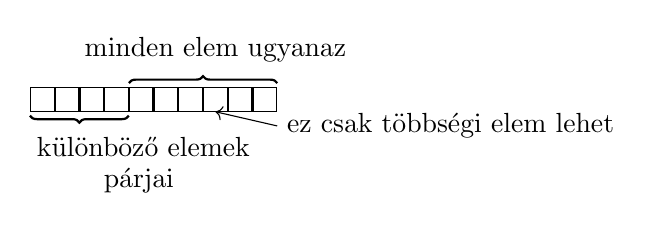
\begin{tikzpicture}[
    squarenode/.style={rectangle, draw=black, minimum width=0.3cm, minimum height=0.3cm},
]
\node[squarenode](a1){};
\node[squarenode](a2)[right = 0cm of a1]{};
\node[squarenode](a3)[right = 0cm of a2]{};
\node[squarenode](a4)[right = 0cm of a3]{};
\node[squarenode](a5)[right = 0cm of a4]{};
\node[squarenode](a6)[right = 0cm of a5]{};
\node[squarenode](a7)[right = 0cm of a6]{};
\node[squarenode](a8)[right = 0cm of a7]{};
\node[squarenode](a9)[right = 0cm of a8]{};
\node[squarenode](a10)[right = 0cm of a9]{};
\draw[thick, decoration={brace, raise=0.05cm, mirror}, decorate] (a1.south west) -- (a4.south east);
\draw[thick, decoration={brace, raise=0.05cm}, decorate] (a5.north west) -- (a10.north east);
\node[below right = 0.2cm and -0.35cm of a1]{különböző elemek};
\node[below right = 0.6cm and 0.5cm of a1]{párjai};
\node[above = 0.2cm of a8]{minden elem ugyanaz};
\node[below right = -0.1cm and 0cm of a10](majority_text){ez csak többségi elem lehet};
\draw[->] (majority_text.west) -- (a8.south);
\end{tikzpicture}

\textbf{Hogyan?}

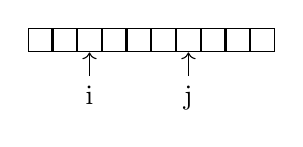
\begin{tikzpicture}[
    squarenode/.style={rectangle, draw=black, minimum width=0.3cm, minimum height=0.3cm},
]
\node[squarenode](a1){};
\node[squarenode](a2)[right = 0cm of a1]{};
\node[squarenode](a3)[right = 0cm of a2]{};
\node[squarenode](a4)[right = 0cm of a3]{};
\node[squarenode](a5)[right = 0cm of a4]{};
\node[squarenode](a6)[right = 0cm of a5]{};
\node[squarenode](a7)[right = 0cm of a6]{};
\node[squarenode](a8)[right = 0cm of a7]{};
\node[squarenode](a9)[right = 0cm of a8]{};
\node[squarenode](a10)[right = 0cm of a9]{};
\node(i)[below = 0.3cm of a3]{i};
\node(j)[below = 0.3cm of a7]{j};
\draw[->] (i) -- (a3);
\draw[->] (j) -- (a7);
\end{tikzpicture}

Tegyük fel, hogy $A[j]$-nél vagyunk, és $A[1:i]$ a párok sora, míg $A[i+1:j]$ homogén.
Ekkor ha $A[j] = A[i+1]$, akkor a homogén részhez hozzávesszük $A[j]$-t.
Ha viszont $A[j] \neq A[i+1]$, akkor megcseréljük $A[j]$-t $A[i+2]$-vel, és ezzel növeljük a párok számát (az első rész 2-vel hosszabb lesz).
Innentől a homogén rész az $A[i+3:j]$.
A rendezés végén ha marad homogén rész, akkor az a többségi elem.

\textbf{Futási idő:} mivel egyszer megyünk végig, ez lineáris, $O(n)$.

\subsubsection*{Mester tétel gyakorlás}

\begin{itemize}
    \item $T(n) = 2T(\frac{n}{2}) + n^3$
    \item $a = 2$, $b = 2$, $f(n) = n^3$
    \item $n^{\log_b a} = n^{\log_2 2} = n^1 = n$
    \item $f(n) = n^3 > n$
\end{itemize}

3. eset:
$f(n) = \Omega(n^{\log_b a + \mathcal{E}}) \rightarrow \mathcal{E}=2$ \checkmark

Regularitás:
\begin{flalign*}
    a f(\frac{n}{b}) &\leq c f(n)&&\\
    2 f(\frac{n}{2}) &\leq c f(n)&&\\
    2 \frac{n^3}{8} &\leq c n^3&&\\
    f(\frac{n^3}{8}) &\leq c n^3&&\\
    \frac{n^3}{4} &\leq c n^3
\end{flalign*}

$c < 1$, $c \geq \frac{1}{4}$ \checkmark

$T(n) = \Theta(f(n)) = \Theta(n^3)$

\clearpage
\section{gyakorlat (2025. október 8.)}
\subsection*{Oszd meg és uralkodj algoritmusok}
\subsubsection*{Geometria}
Adott $n$ pont a síkon. Határozzuk meg
\begin{enumerate}
    \item a két legközelebbit
    \item a két legtávolabbit.
\end{enumerate}

Kicsit távolabbról indulunk.

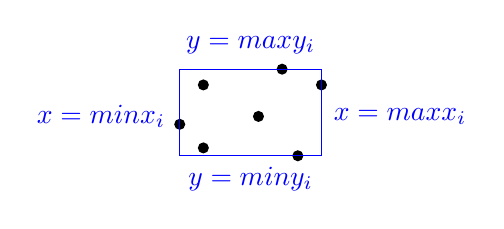
\begin{tikzpicture}
\fill (0, 0) circle(2pt);
\fill (0.3, 0.5) circle(2pt);
\fill (0.3, -0.3) circle(2pt);
\fill (1, 0.1) circle(2pt);
\fill (1.3, 0.7) circle(2pt);
\fill (1.5, -0.4) circle(2pt);
\fill (1.8, 0.5) circle(2pt);
\draw[blue] (0, -0.4) -- (0, 0.7);
\draw[blue] (0, -0.4) -- (1.8, -0.4);
\draw[blue] (1.8, 0.7) -- (1.8, -0.4);
\draw[blue] (0, 0.7) -- (1.8, 0.7);
\node at (-1, 0.1) {\color{blue}{$x = min x_i$}};
\node at (2.8, 0.1) {\color{blue}{$x = max x_i$}};
\node at (0.9, -0.7) {\color{blue}{$y = min y_i$}};
\node at (0.9, 1) {\color{blue}{$y = max y_i$}};

\end{tikzpicture}

$(x_1, y_1), (x_2, y_2), \cdots, (x_n, y_n)$ a pontok.
\setulcolor{blue}
Határozzuk meg a legkisebb olyan \ul{téglalapot} amelynek oldalai párhuzamosak a koordinátatengelyekkel és az összes pontot tartalmazza.
\setulcolor{black}

Két min és két max számolás $\rightarrow 4n-4$ összehasonlítás.
Lehet kevesebbel is?
Egyszerre $min x_i$ és $max x_i$, illetve $min y_i$ és $max y_i$?
Lássuk a $min x_i$ és $max x_i$ esetet:

$\underbrace{x_1, x_2}, \underbrace{x_3, x_4}, \underbrace{x_5, x_6}, \cdots, x_{n-2}, \underbrace{x_{n-1}, x_n}$

Az egyszerűség kedvéért tegyük fel, hogy az értékek páronként különbözőek.

Ha $x_1 < x_2$, akkor $x_1 \neq max x_i$ és $x_2 \neq min x_i \Rightarrow \left[\frac{n}{2}\right]$ összehasonlítással a feladat visszavezethető $\left\lceil\frac{n}{2}\right\rceil$ szám közül a maximum és a minimum meghatározására.
Ezzel az összehasonlítások számát $\left[\frac{n}{2}\right]$-vel tudtuk csökkenteni.
Igazából nem számít, ha az elemek között vannak megegyezőek.

Legkisebb téglalap $\rightarrow$ legkisebb sokszög (amely az összes pontot tartalmazza).

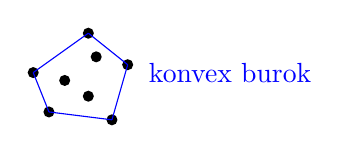
\begin{tikzpicture}
\fill (0, 0) circle(2pt);
\fill (0.2, -0.5) circle(2pt);
\fill (1, -0.6) circle(2pt);
\fill (1.2, 0.1) circle(2pt);
\fill (0.7, 0.5) circle(2pt);
\draw[blue](0, 0) -- (0.2, -0.5);
\draw[blue](0.2, -0.5) -- (1, -0.6);
\draw[blue](1, -0.6) -- (1.2, 0.1);
\draw[blue](1.2, 0.1) -- (0.7, 0.5);
\draw[blue](0.7, 0.5) -- (0, 0);
\fill (0.4, -0.1) circle(2pt);
\fill (0.7, -0.3) circle(2pt);
\fill (0.8, 0.2) circle(2pt);
\node at (2.5, 0) {\color{blue}{konvex burok}};
\end{tikzpicture}

Nem nehéz belátni, hogy a két legtávolabbi pont a konvex burok két csúcsa.

\setulcolor{blue}
Az első lépés a két legtávolabbi pont meghatározásához a \ul{konvex burok meghatározása}.
\setulcolor{black}

$(x_1, y_1), (x_2, y_2), \cdots, (x_n, y_n) \rightarrow$ a konvex burok csúcsainak felsorolása a konvex burkon az óramutató járása szerint.

Milyen "bonyolult" a konvex burok meghatározása?
Legalább annyira, mint a rendezés.

$(x_1, x_1^2), (x_2, x_2^2), \cdots, (x_n, x_n^2)$ bemenethez:

\begin{tikzpicture}
\begin{axis}[
    axis lines=middle,
    ymin=-2, ymax=8,
    xmin=-1, xmax=4,
    restrict x to domain=-0.1:2.5,
    xticklabel=\empty,
    yticklabel=\empty,
    xtick=\empty,
    ytick=\empty
]
    \addplot[mark=none] {pow(x,2)} node[right]{$y=x^2$};
\end{axis}

\node[orange] at (2, 0.9) {$x_{i_1}$};
\node[orange] at (2.5, 0.9) {$x_{i_2}$};
\node[orange] at (3, 0.9) {$x_{i_3}$};
\node[orange] at (4, 0.9) {$\cdots$};

\fill[orange] (2, 1.25) circle(2pt);
\fill[orange] (2.5, 1.52) circle(2pt);
\fill[orange] (3, 1.95) circle(2pt);
\fill[orange] (3.5, 2.52) circle(2pt);
\fill[orange] (4, 3.25) circle(2pt);
\fill[orange] (4.5, 4.12) circle(2pt);

\draw[orange] (2, 1.15) -- (2, 1.25);
\draw[orange] (2.5, 1.15) -- (2.5, 1.52);
\draw[orange] (3, 1.15) -- (3, 1.95);
\draw[orange] (3.5, 1.15) -- (3.5, 2.52);
\draw[orange] (4, 1.15) -- (4, 3.25);
\draw[orange] (4.5, 1.15) -- (4.5, 4.12);

\draw[red] (2, 1.25) -- (4.5, 4.12);
\node[red] at (3, 2.9) {\lcirclearrowright};
\end{tikzpicture}

\clearpage
Egy konvex burok algoritmus rendezi is az $x_1, x_2, \cdots, x_n$ számokat (csökkenően).
$\mathcal{O}(n \log n)$ költségűek a "jó" konvex burok algoritmusok.
Több ilyen is van, oszd meg és uralkodj is:

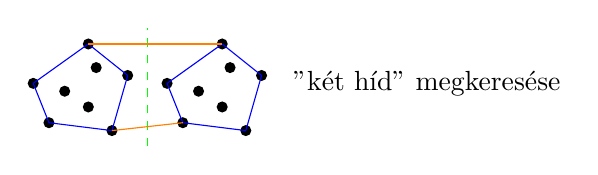
\begin{tikzpicture}
\fill (0, 0) circle(2pt);
\fill (0.2, -0.5) circle(2pt);
\fill (1, -0.6) circle(2pt);
\fill (1.2, 0.1) circle(2pt);
\fill (0.7, 0.5) circle(2pt);
\draw[blue](0, 0) -- (0.2, -0.5);
\draw[blue](0.2, -0.5) -- (1, -0.6);
\draw[blue](1, -0.6) -- (1.2, 0.1);
\draw[blue](1.2, 0.1) -- (0.7, 0.5);
\draw[blue](0.7, 0.5) -- (0, 0);
\fill (0.4, -0.1) circle(2pt);
\fill (0.7, -0.3) circle(2pt);
\fill (0.8, 0.2) circle(2pt);

\draw[green, dashed] (1.45, -0.8) -- (1.45, 0.7);

\fill (1.7, 0) circle(2pt);
\fill (1.9, -0.5) circle(2pt);
\fill (2.7, -0.6) circle(2pt);
\fill (2.9, 0.1) circle(2pt);
\fill (2.4, 0.5) circle(2pt);
\draw[blue](1.7, 0) -- (1.9, -0.5);
\draw[blue](1.9, -0.5) -- (2.7, -0.6);
\draw[blue](2.7, -0.6) -- (2.9, 0.1);
\draw[blue](2.9, 0.1) -- (2.4, 0.5);
\draw[blue](2.4, 0.5) -- (1.7, 0);
\fill (2.1, -0.1) circle(2pt);
\fill (2.4, -0.3) circle(2pt);
\fill (2.5, 0.2) circle(2pt);

\draw[orange] (0.7, 0.5) -- (2.4, 0.5);
\draw[orange] (1, -0.6) -- (1.9, -0.5);
\node at (5, 0){"két híd" megkeresése};
\end{tikzpicture}

\begin{enumerate}
    \item két feleakkora feladat
    \item rekurzívan megoldjuk a részfeladatokat
    \item "egyesítjük" a két konvex burkot (két híd)
\end{enumerate}

Ezek után a két legtávolabbi csúcs a konvex burkon (nem oszd meg és uralkodj algoritmus):

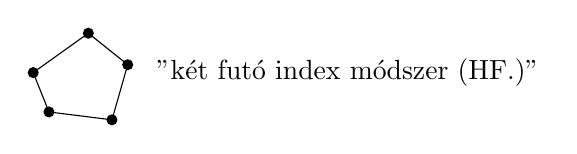
\begin{tikzpicture}
\fill (0, 0) circle(2pt);
\fill (0.2, -0.5) circle(2pt);
\fill (1, -0.6) circle(2pt);
\fill (1.2, 0.1) circle(2pt);
\fill (0.7, 0.5) circle(2pt);
\draw(0, 0) -- (0.2, -0.5);
\draw(0.2, -0.5) -- (1, -0.6);
\draw(1, -0.6) -- (1.2, 0.1);
\draw(1.2, 0.1) -- (0.7, 0.5);
\draw(0.7, 0.5) -- (0, 0);
\node at (4, 0){"két futó index módszer (HF.)"};
\end{tikzpicture}

\subsubsection*{Minimális távolság}

\textbf{Oszd meg és uralkodj algoritmus}

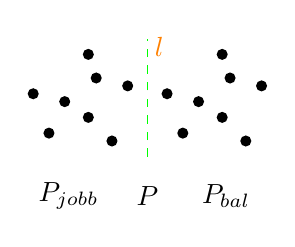
\begin{tikzpicture}
\fill (0, 0) circle(2pt);
\fill (0.2, -0.5) circle(2pt);
\fill (1, -0.6) circle(2pt);
\fill (1.2, 0.1) circle(2pt);
\fill (0.7, 0.5) circle(2pt);
\fill (0.4, -0.1) circle(2pt);
\fill (0.7, -0.3) circle(2pt);
\fill (0.8, 0.2) circle(2pt);

\fill (1.7, 0) circle(2pt);
\fill (1.9, -0.5) circle(2pt);
\fill (2.7, -0.6) circle(2pt);
\fill (2.9, 0.1) circle(2pt);
\fill (2.4, 0.5) circle(2pt);
\fill (2.1, -0.1) circle(2pt);
\fill (2.4, -0.3) circle(2pt);
\fill (2.5, 0.2) circle(2pt);

\draw[green, dashed] (1.45, -0.8) -- (1.45, 0.7);

\node at (1.6, 0.6){\color{orange} $l$};
\node at (1.45, -1.3){$P$};
\node at (2.45, -1.3){$P_{bal}$};
\node at (0.45, -1.3){$P_{jobb}$};
\end{tikzpicture}

\begin{enumerate}
    \item két feleakkora feladatra bontás $\rightarrow P_{bal}, P_{jobb}$
    \item rekurzívan meghatározzuk a minimális távolságot $P_{bal}$-ban és $P_{jobb}$-ban:
    \begin{itemize}
        \item $P_{bal} \rightarrow \delta_{bal}$
        \item $P_{jobb} \rightarrow \delta_{jobb}$
    \end{itemize}
    \item minimális távolság meghatározása
\end{enumerate}

A minimális távolság vagy baloldalon vagy jobboldalon van, vagy keresztezi az $l$ felező egyenest.

A harmadik esetben $l$-től nem túl messze lévő pontokra elég szorítkozni.\\
Legyen $\delta = min(\delta_{bal}, \delta_{jobb})$.

\begin{tikzpicture}
\draw (0, 0) -- (0, 4);
\draw (2, 0) -- (2, 4);
\draw[dashed] (1, 0) -- (1, 4);

\node at (1.3, 3.6){$l$};

\draw[->] (0, 0.5) -- (1, 0.5);
\draw[->] (1, 0.5) -- (0, 0.5);
\draw[->] (1, 0.5) -- (2, 0.5);
\draw[->] (2, 0.5) -- (1, 0.5);

\node at (0.5, 0.25){$\delta$};
\node at (1.5, 0.25){$\delta$};
\end{tikzpicture}

Ebben a $\delta$ sugarú sávban kell a két pontnak lenni, amelyek a min távolságot minimalizálják.

\clearpage
Itt van még valami, amit érdemes észrevenni.
Tekintsük a sávbeli pontokat az $y$ koordinátájuk szerint monoton növekvően rendezetten.

\begin{tikzpicture}
\draw (0, 0) -- (0, 4);
\draw (2, 0) -- (2, 4);
\draw (1, 0) -- (1, 4);

\draw[->] (0, 0.5) -- (1, 0.5);
\draw[->] (1, 0.5) -- (0, 0.5);
\draw[->] (1, 0.5) -- (2, 0.5);
\draw[->] (2, 0.5) -- (1, 0.5);

\node at (0.5, 0.25){$\delta$};
\node at (1.5, 0.25){$\delta$};

\draw[blue] (0, 1.5) -- (2, 1.5);
\draw[blue] (0, 2.5) -- (2, 2.5);
\draw[blue, ->] (-0.25, 1.5) -- (-0.25, 2.5);
\draw[blue, ->] (-0.25, 2.5) -- (-0.25, 1.5);
\node[blue] at (-0.5, 2){$\delta$};
\fill (0.5, 1.5) circle(2pt);
\node at (6, 1){"első pont" $\rightarrow$ hány ponttól lehet $\delta$-nál közelebb?};
\draw[-Latex] (2.2, 1) -- (0.5, 1.5);
\end{tikzpicture}

Minden ilyen pont szükségképpen ebben a téglalapban van:

\begin{tikzpicture}
\draw[blue] (0, 0) -- (4, 0);
\draw[blue] (0, 2) -- (4, 2);
\draw (2, 0) -- (2, 2);
\draw (0, 0) -- (0, 2);
\draw (4, 0) -- (4, 2);
\draw[dashed] (0, 1) -- (4, 1);
\draw[dashed] (1, 0) -- (1, 2);
\draw[dashed] (3, 0) -- (3, 2);

\node at (-0.3, 1){$\delta$};
\node at (1, -0.3){$\delta$};
\node at (3, -0.3){$\delta$};

\fill (0.7, 0) circle(2pt);
\end{tikzpicture}

Tekintsük a fenti 8 kis négyzetet.
Mivel ezek átmérője $\frac{8}{2} \sqrt{2} = \frac{8}{\sqrt{2}} < \delta$, és az $l$ bal, illetve jobb oldalán a minimális távolság legalább $\delta$, így a 8 kis négyzet egyikében sem lehet egynél több $P$-beli pont.
Így a legalsó ponttól $\delta$-nál kisebb távolságra csak a következő 7 pont valamelyike lehet.
Felfelé haladva ez mindig igaz lesz.

Költség: $T(n) = 2T(\frac{n}{2}) + \underbrace{\mathcal{O}(n \log n)}_{\text{rendezések}} \rightarrow T(n) ( \mathcal{O}(n \log^2 n))$

$\mathcal{O}(n \log^2 n) \rightarrow \mathcal{O}(n \log n)$


Előfeldolgozás $\rightarrow$ előrendezés (x és y koordináták szerint is) $\rightarrow$ rekurzív hívásokban már csak kiválogatás

$T(n) = 2T(\frac{n}{2}) + \mathcal{O}(n) \rightarrow T(n) = \mathcal{O}(n \log n)$
\clearpage
\section{gyakorlat (2025. október 15.)}
\subsubsection*{Még egy geometriai oszd meg és uralkodj algoritmus (igazából összefésülés variáció)}
\begin{figure}[H]
  \includegraphics[width=5cm]{gy/img/gy06_skyline1}
\end{figure}
$n$ téglalap, amelyek az $x$ tengelyen állnak

Feladat: sziluett (felső burkoló töröttvonal) meghatározása.

Téglalapok: $T_1, T_2, \cdots, T_n$

\begin{tikzpicture}
\draw[->] (-0.5, 0) -- (4, 0);
\draw[->] (0, -0.5) -- (0, 3);

\draw[dashed] (0, 2) -- (1, 2);
\draw (1, 2) -- (2, 2);
\draw (1, 0) -- (1, 2); 
\draw (2, 0) -- (2, 2);

\node at (-0.3, 2){$y_i$};
\node at (1, -0.3){$x'_i$};
\node at (2, -0.3){$x''_i$};
\node at (1.5, 1){$T_i$};
\node at (4, 1){$T_i \leftrightarrow (x'_i, y_i, x''_i)$};
\end{tikzpicture}

Sziluett

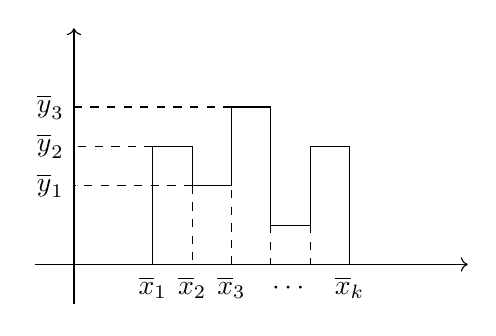
\begin{tikzpicture}
\draw[->] (-0.5, 0) -- (5, 0);
\draw[->] (0, -0.5) -- (0, 3);

\draw (1, 0) -- (1, 1.5);
\draw (1, 1.5) -- (1.5, 1.5);
\draw (1.5, 1.5) -- (1.5, 1);
\draw (1.5, 1) -- (2, 1);
\draw (2, 1) -- (2, 2);
\draw (2, 2) -- (2.5, 2);
\draw (2.5, 2) -- (2.5, 0.5);
\draw (2.5, 0.5) -- (3, 0.5);
\draw (3, 0.5) -- (3, 1.5);
\draw (3, 1.5) -- (3.5, 1.5);
\draw (3.5, 1.5) -- (3.5, 0);

\draw[dashed] (2, 2) -- (0, 2);
\draw[dashed] (2, 2) -- (2, 0);
\draw[dashed] (1, 1.5) -- (0, 1.5);
\draw[dashed] (1, 1.5) -- (1, 0);
\draw[dashed] (1.5, 1) -- (0, 1);
\draw[dashed] (1.5, 1) -- (1.5, 0);
\draw[dashed] (2.5, 0.5) -- (2.5, 0);
\draw[dashed] (3, 0.5) -- (3, 0);

\node at (-0.3, 2){$\overline{y}_3$};
\node at (-0.3, 1.5){$\overline{y}_2$};
\node at (-0.3, 1){$\overline{y}_1$};

\node at (1, -0.3){$\overline{x}_1$};
\node at (1.5, -0.3){$\overline{x}_2$};
\node at (2, -0.3){$\overline{x}_3$};
\node at (2.75, -0.3){$\cdots$};
\node at (3.5, -0.3){$\overline{x}_k$};
\end{tikzpicture}

$(\overline{x}_1, \overline{y}_1, \overline{x}_2, \overline{y}_2, \cdots, \overline{y}_{k-1}, \overline{x}_k)$

\textbf{Oszd meg és uralkodj algoritmus}\\
\begin{enumerate}
    \item Két feleakkora méretű részfeladat
    \begin{itemize}
    \item $T_1 ,T_2, \cdots, T_{n/2}$ sziluettjének meghatározása
    \item $T_{n/2 + 1} ,T_{n/2 + 2}, \cdots, T_{n}$ sziluettjének meghatározása
    \end{itemize}
    \item Rekurzívan megoldjuk a részfeladatokat (egy téglalap esetén triviális)
    \item Összekombináljuk a két sziluettet:
    \begin{figure}[H]
        \includegraphics[width=5cm]{gy/img/gy06_skyline2}
    \end{figure}
    (ez már egy összefésülés)
\end{enumerate}
Minden szakaszon a magasabban fekvő szakaszt választjuk a két sziluetten.


Implementáljuk ezt ha tényleg minden részletében érteni szeretnénk.

Költség: $T(n) = 2T(\frac{n}{2}) + \mathcal{O}(n) \rightarrow T(n) = \mathcal(O)(n \log n)$


\subsection{Érmék egy sorban (tegnapi előadás)}
(Ez már nem oszd meg és uralkodj)

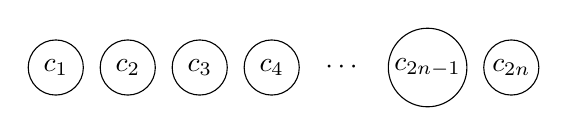
\begin{tikzpicture}[
    roundnode/.style={circle, draw=black, minimum size=0.7cm, inner sep=0.5mm}
]
\node[roundnode](c1){$c_1$};
\node[roundnode](c2)[right = 0.2cm of c1]{$c_2$};
\node[roundnode](c3)[right = 0.2cm of c2]{$c_3$};
\node[roundnode](c4)[right = 0.2cm of c3]{$c_4$};
\node(cdots)[right = 0.2cm of c4]{$\cdots$};
\node[roundnode](c2n1)[right = 0.2cm of cdots]{$c_{2n-1}$};
\node[roundnode](c2n)[right = 0.2cm of c2n1]{$c_{2n}$};   
\end{tikzpicture}

Egy sorban $2n$ (nem feltétlenül páronként) különböző érmék vannak.
Két játékos felváltva elvesz a (megmaradt) érmék sorának valamelyik végéről egy érmét.
Az győz, akinél az elvett érmék értékének összege nagyobb.

Először is: döntetlen lehetséges.
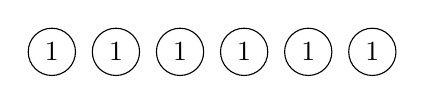
\begin{tikzpicture}[
    roundnode/.style={circle, draw=black, minimum size=0.6cm, inner sep=0.5mm}
]
\node[roundnode](c1){$1$};
\node[roundnode](c2)[right = 0.2cm of c1]{$1$};
\node[roundnode](c3)[right = 0.2cm of c2]{$1$};
\node[roundnode](c4)[right = 0.2cm of c3]{$1$};
\node[roundnode](c5)[right = 0.2cm of c4]{$1$};
\node[roundnode](c6)[right = 0.2cm of c5]{$1$};
\end{tikzpicture}

A nyerő stratégia a nem vesztő stratégia.

Nyerő stratégia a kezdő számára: tud úgy érmét elvenni először, hogy erre "bármit lép" a másik játékos, a kezdő megint tud úgy érmét elvenni, hogy erre "bármit lép" a másik játékos, \cdots, a kezdő nyer (nem veszít)

Nyerő stratégia a másik játékosnak: bármit lép a kezdő játékos, a másik játékos tud úgy érmét elvenni, hogy erre bármit lép a kezdő játékos, a másik tud úgy érmét elvenni, \cdots, a másik játékos nyer (nem veszít).

Ebben a játékban a kezdőnek van nyerő (nem vesztő) stratégiája!

\setstcolor{black}
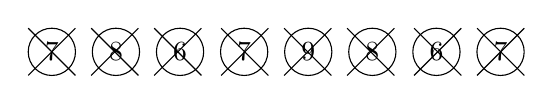
\begin{tikzpicture}[
    roundnode/.style={circle, draw=black, minimum size=0.6cm, inner sep=0.5mm}
]
\node[roundnode](c1){$7$};
\node[roundnode](c2)[right = 0.2cm of c1]{$8$};
\node[roundnode](c3)[right = 0.2cm of c2]{$6$};
\node[roundnode](c4)[right = 0.2cm of c3]{$7$};
\node[roundnode](c5)[right = 0.2cm of c4]{$9$};
\node[roundnode](c6)[right = 0.2cm of c5]{$8$};
\node[roundnode](c7)[right = 0.2cm of c6]{$6$};
\node[roundnode](c8)[right = 0.2cm of c7]{$7$};

\draw (-0.3, -0.3) -- ++(0.6, 0.6);
\draw (-0.3, 0.3) -- ++(0.6, -0.6);

\draw (0.5, -0.3) -- ++(0.6, 0.6);
\draw (0.5, 0.3) -- ++(0.6, -0.6);

\draw (1.3, -0.3) -- ++(0.6, 0.6);
\draw (1.3, 0.3) -- ++(0.6, -0.6);

\draw (2.15, -0.3) -- ++(0.6, 0.6);
\draw (2.15, 0.3) -- ++(0.6, -0.6);

\draw (2.95, -0.3) -- ++(0.6, 0.6);
\draw (2.95, 0.3) -- ++(0.6, -0.6);

\draw (3.75, -0.3) -- ++(0.6, 0.6);
\draw (3.75, 0.3) -- ++(0.6, -0.6);

\draw (4.6, -0.3) -- ++(0.6, 0.6);
\draw (4.6, 0.3) -- ++(0.6, -0.6);

\draw (5.4, -0.3) -- ++(0.6, 0.6);
\draw (5.4, 0.3) -- ++(0.6, -0.6);
\end{tikzpicture}

Kezdő (összesen 30):
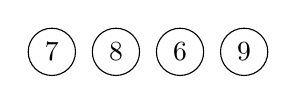
\begin{tikzpicture}[
    roundnode/.style={circle, draw=black, minimum size=0.6cm, inner sep=0.5mm}
]
\node[roundnode](c1){$7$};
\node[roundnode](c2)[right = 0.2cm of c1]{$8$};
\node[roundnode](c3)[right = 0.2cm of c2]{$6$};
\node[roundnode](c4)[right = 0.2cm of c3]{$9$};
\end{tikzpicture}

Másik (összesen 28):
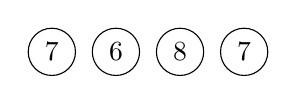
\begin{tikzpicture}[
    roundnode/.style={circle, draw=black, minimum size=0.6cm, inner sep=0.5mm}
]
\node[roundnode](c1){$7$};
\node[roundnode](c2)[right = 0.2cm of c1]{$6$};
\node[roundnode](c3)[right = 0.2cm of c2]{$8$};
\node[roundnode](c4)[right = 0.2cm of c3]{$7$};
\end{tikzpicture}

A kezdő játékos ki tudja kényszeríteni, hogy a másik csak a páros indexű $c_i$-ket és azt is hogy csak a páratlan indexű $c_i$-ket vegye el (az összeset).

Pl. a páros indexekre:

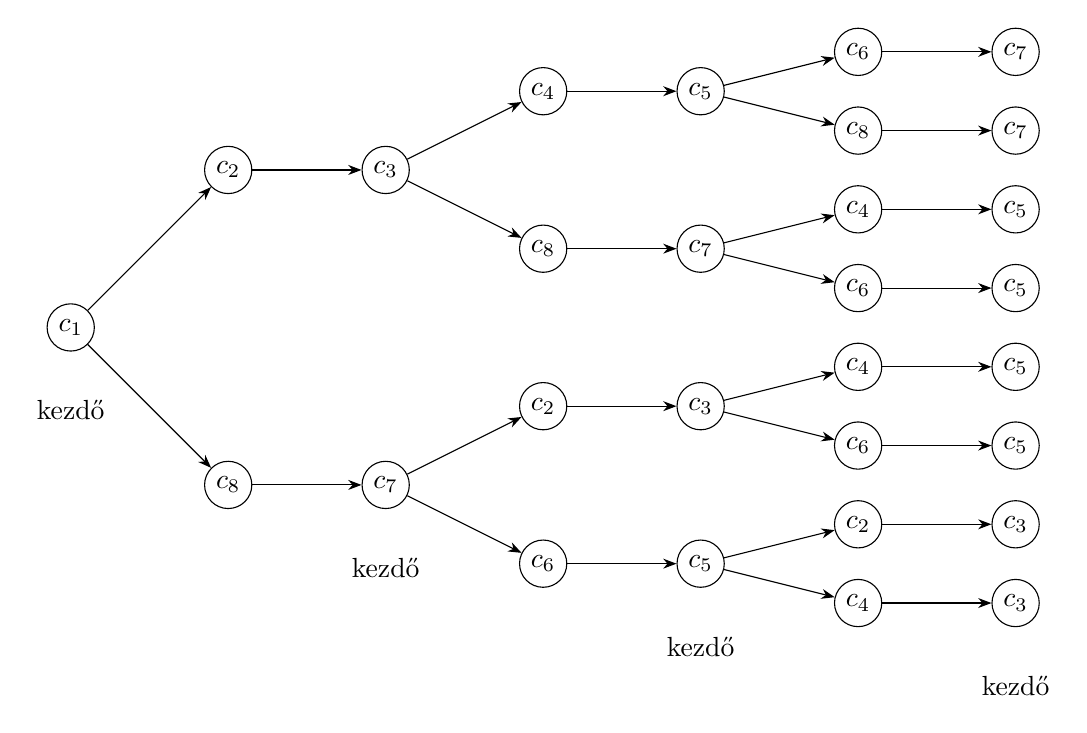
\begin{tikzpicture}[
    roundnode/.style={circle, draw=black, minimum size=0.6cm, inner sep=0.5mm}
]
\node[roundnode](c1_1) at (0, 0) {$c_1$};

\node[roundnode](c2_1) at (2, 2) {$c_2$};
\node[roundnode](c2_2) at (2, -2) {$c_8$};

\node[roundnode](c3_1) at (4, 2) {$c_3$};
\node[roundnode](c3_2) at (4, -2) {$c_7$};

\node[roundnode](c4_1) at (6, 3) {$c_4$};
\node[roundnode](c4_2) at (6, 1) {$c_8$};
\node[roundnode](c4_3) at (6, -1) {$c_2$};
\node[roundnode](c4_4) at (6, -3) {$c_6$};

\node[roundnode](c5_1) at (8, 3) {$c_5$};
\node[roundnode](c5_2) at (8, 1) {$c_7$};
\node[roundnode](c5_3) at (8, -1) {$c_3$};
\node[roundnode](c5_4) at (8, -3) {$c_5$};

\node[roundnode](c6_1) at (10, 3.5) {$c_6$};
\node[roundnode](c6_2) at (10, 2.5) {$c_8$};
\node[roundnode](c6_3) at (10, 1.5) {$c_4$};
\node[roundnode](c6_4) at (10, 0.5) {$c_6$};
\node[roundnode](c6_5) at (10, -0.5) {$c_4$};
\node[roundnode](c6_6) at (10, -1.5) {$c_6$};
\node[roundnode](c6_7) at (10, -2.5) {$c_2$};
\node[roundnode](c6_8) at (10, -3.5) {$c_4$};

\node[roundnode](c7_1) at (12, 3.5) {$c_7$};
\node[roundnode](c7_2) at (12, 2.5) {$c_7$};
\node[roundnode](c7_3) at (12, 1.5) {$c_5$};
\node[roundnode](c7_4) at (12, 0.5) {$c_5$};
\node[roundnode](c7_5) at (12, -0.5) {$c_5$};
\node[roundnode](c7_6) at (12, -1.5) {$c_5$};
\node[roundnode](c7_7) at (12, -2.5) {$c_3$};
\node[roundnode](c7_8) at (12, -3.5) {$c_3$};

\draw[-Stealth] (c1_1) -- (c2_1);
\draw[-Stealth] (c1_1) -- (c2_2);

\draw[-Stealth] (c2_1) -- (c3_1);
\draw[-Stealth] (c2_2) -- (c3_2);

\draw[-Stealth] (c3_1) -- (c4_1);
\draw[-Stealth] (c3_1) -- (c4_2);
\draw[-Stealth] (c3_2) -- (c4_3);
\draw[-Stealth] (c3_2) -- (c4_4);

\draw[-Stealth] (c4_1) -- (c5_1);
\draw[-Stealth] (c4_2) -- (c5_2);
\draw[-Stealth] (c4_3) -- (c5_3);
\draw[-Stealth] (c4_4) -- (c5_4);

\draw[-Stealth] (c5_1) -- (c6_1);
\draw[-Stealth] (c5_1) -- (c6_2);
\draw[-Stealth] (c5_2) -- (c6_3);
\draw[-Stealth] (c5_2) -- (c6_4);
\draw[-Stealth] (c5_3) -- (c6_5);
\draw[-Stealth] (c5_3) -- (c6_6);
\draw[-Stealth] (c5_4) -- (c6_7);
\draw[-Stealth] (c5_4) -- (c6_8);

\draw[-Stealth] (c6_1) -- (c7_1);
\draw[-Stealth] (c6_2) -- (c7_2);
\draw[-Stealth] (c6_3) -- (c7_3);
\draw[-Stealth] (c6_4) -- (c7_4);
\draw[-Stealth] (c6_5) -- (c7_5);
\draw[-Stealth] (c6_6) -- (c7_6);
\draw[-Stealth] (c6_7) -- (c7_7);
\draw[-Stealth] (c6_8) -- (c7_8);

\node[below=0.5cm of c1_1]{kezdő};
\node[below=0.5cm of c3_2]{kezdő};
\node[below=0.5cm of c5_4]{kezdő};
\node[below=0.5cm of c7_8]{kezdő};
\end{tikzpicture}


Ezek után a nyerő stratégia:\\
$S_{ps} := c_2 + c_4 + c_6 + \cdots + c_{2n}$\\
$S_{plan} := c_1 + c_3 + c_5 + \cdots + c_{2n-1}$

Ha $S_{ps} \leq S_{plan}$, akkor a kezdő mindig a páratlan indexű érméket vegye el, különben mindig a páros indexűeket.

Példánkban:\\
$S_{ps} = 8 + 7 + 8 + 7 = 30$\\
$S_{plan} = 7 + 6 + 9 + 6 = 28$\\
A kezdőnek a páros indexű érméket kell elvenni.

Optimális ez?
Nem feltétlenül.\\
Új kérdés: milyen stratégiát kövessen a kezdő, hogy a különbség a javára maximális legyen?
Az előző példánál a második játékosnak (globálisan) nem volt mozgástere.
Általában ez nincs így.

Optimális stratégia a kezdő számára: bárhogy játszik a másik, a különbség mindenképp meglesz.
Aprópénzre váltva: a másik "optimális stratégiája" mellett is (a másik játékos optimális stratégiája: minimalizálni akarja a különbséget).




\clearpage
\section{gyakorlat (2025. október 22.)}
\subsection{Dinamikus programozás}
\subsubsection*{Mátrixok optimális zárójelezése}
$A_1 A_2 \cdots A_n$\\
A szorzat nem függ a zárójelezéstől, de a kiszámításhoz szükséges elemi szorzások száma általában nagyon is.

\sethlcolor{orange}
\textbf{Példa} \hl{(zh. feladat)}:

Mátrixok:
\begin{flalign*}
    &A_1: 25 \times 30 &&\\
    &A_2: 30 \times 10 &&\\
    &A_3: 10 \times 5 &&\\
    &A_4: 5 \times 10 &&\\
    &A_5: 10 \times 15 &&\\
    &A_6: 15 \times 20 &&
\end{flalign*}
Dimenziók ($A_1 A_2 A_3 A_4 A_5 A_6$ sorrend alapján sorban):
\begin{flalign*}
    &q_0 = 25 &&\\
    &q_1 = 30 &&\\
    &q_2 = 10 &&\\
    &q_3 = 5  &&\\
    &q_4 = 10 &&\\
    &q_5 = 15 &&\\
    &q_6 = 20 &&
\end{flalign*}
Feladat: $A_1 A_2 A_3 A_4 A_5 A_6$ optimális zárójelezése.

Megoldás: két $6 \times 6$-os táblázat

\begin{tabular}{c c}
    \includegraphics[width=6cm]{gy/img/gy07_table_l.pdf} & \includegraphics[width=6cm]{gy/img/gy07_table_k.pdf} \\
    $l[i,j]$ & $k[i,j]$ ("az a bizonyos $k$") \\
\end{tabular}

\begin{tabular}{l l}
    $l[1,1] = 0$ & $l[1,2] = min\left\{l[1,1] + l[2,2] + q_0 + q_1 + q_2 \right\} = 0 + 0 + 25 \times 30 \times 10 = 7500$ \\
    $l[2,2] = 0$ & $l[2,3] = 30 \times 10 \times 5 = 1500$  \\
    $l[3,3] = 0$ & $l[3,4] = 10 \times 5 \times 10 = 500$   \\
    $l[4,4] = 0$ & $l[4,5] = 5 \times 10 \times 15 = 750$   \\
    $l[5,5] = 0$ & $l[5,6] = 10 \times 15 \times 20 = 3000$ \\
    $l[6,6] = 0$ &                                          \\
\end{tabular}

\textbf{Általános formula:}\\
$l[i,j] = \underset{i \leq k \leq j-1}{min} \{ l[i,k] + l[k+1, j] + \underbrace{q_{i-1} q_k q_j}_{\text{dimenziók}} \}$\\
$k[i,j] = $ az a k, ahol a fenti zárójeles összeg a legkisebb.

\clearpage
\textbf{1. lépés: "átlós kitöltés":} amikor egy adott $l[i,j]$-t számítjuk, már minden $l[i,k]$ (a sorban előtte lévők) és $l[k+1, j]$ (az oszlopban alatta lévők) ismert.

\begin{flalign*}
&l[1,3] = min 
\begin{Bmatrix}
    l[1,\text{\fbox{$1$}}] + l[2,3] + 25 \cdot 30 \cdot 5 = \text{\fbox{$5250$}} \\
    l[1,2] + l[3,3] + 25 \cdot 10 \cdot 5 = 8750
\end{Bmatrix}&&
\end{flalign*}

\begin{flalign*}
&l[2,4] = min 
\begin{Bmatrix}
    l[2,2] + l[3,4] + 30 \cdot 10 \cdot 10 = 3500 \\
    l[2,\text{\fbox{$3$}}] + l[4,4] + 30 \cdot 5 \cdot 10 = \text{\fbox{$3000$}}
\end{Bmatrix}&&
\end{flalign*}

\begin{flalign*}
&l[3,5] = min 
\begin{Bmatrix}
    l[3,\text{\fbox{$3$}}] + l[4,5] + 10 \cdot 5 \cdot 15 = \text{\fbox{$1500$}} \\
    l[3,4] + l[5,5] + 10 \cdot 10\cdot 15 = 2000
\end{Bmatrix}&&
\end{flalign*}

\begin{flalign*}
&l[4,6] = min 
\begin{Bmatrix}
    l[4,4] + l[5,6] + 5 \cdot 10 \cdot 20 = 4000 \\
    l[4,\text{\fbox{$5$}}] + l[6,6] + 5 \cdot 15 \cdot 20 = \text{\fbox{$2250$}}
\end{Bmatrix}&&
\end{flalign*}

\begin{flalign*}
&l[1,4] = min 
\begin{Bmatrix}
    l[1,1] + l[2,4] + 25 \cdot 30 \cdot 10 = 10500 \\
    l[1,2] + l[3,4] + 25 \cdot 10 \cdot 10 = 10500 \\
    l[1,\text{\fbox{$3$}}] + l[4,4] + 25 \cdot 5 \cdot 10 = \text{\fbox{$6500$}}
\end{Bmatrix}&&
\end{flalign*}
Ha minden sor egyenlő, akkor bármelyiket választhatjuk minimumnak, majd a backtracking során látjuk, hogy ekkor több optimális zárójelezés is létezik.

\begin{flalign*}
&l[2,5] = min 
\begin{Bmatrix}
    l[2,2] + l[3,5] + 30 \cdot 10 \cdot 15 = 6000 \\
    l[2,\text{\fbox{$3$}}] + l[4,5] + 30 \cdot 5 \cdot 15 = \text{\fbox{$4500$}} \\
    l[2,4] + l[5,5] + 30 \cdot 10 \cdot 15 = 7500
\end{Bmatrix}&&
\end{flalign*}

\begin{flalign*}
&l[3,6] = min 
\begin{Bmatrix}
    l[3,\text{\fbox{$3$}}] + l[4,6] + 10 \cdot 5 \cdot 20 = \text{\fbox{$3250$}} \\
    l[3,4] + l[5,6] + 10 \cdot 10 \cdot 20 = 5500 \\
    l[3,5] + l[6,6] + 10 \cdot 15 \cdot 20 = 4500
\end{Bmatrix}&&
\end{flalign*}

\begin{flalign*}
&l[1,5] = min 
\begin{Bmatrix}
    l[1,1] + l[2,5] + 25 \cdot 30 \cdot 15 = 15750 \\
    l[1,2] + l[3,5] + 25 \cdot 10 \cdot 15 = 12750 \\
    l[1,\text{\fbox{$3$}}] + l[4,5] + 25 \cdot 5 \cdot 15 = \text{\fbox{$7875$}} \\
    l[1,4] + l[5,5] + 25 \cdot 10 \cdot 15 = 10250
\end{Bmatrix}&&
\end{flalign*}

\begin{flalign*}
&l[2,6] = min 
\begin{Bmatrix}
    l[2,2] + l[3,6] + 30 \cdot 10 \cdot 20 =  9250 \\
    l[2,\text{\fbox{$3$}}] + l[4,6] + 30 \cdot 5 \cdot 20 = \text{\fbox{$6750$}} \\
    l[2,4] + l[5,6] + 30 \cdot 10 \cdot 20 = 12000 \\
    l[2,5] + l[6,6] + 30 \cdot 15 \cdot 20 = 13500
\end{Bmatrix}&&
\end{flalign*}

\begin{flalign*}
&l[1,6] = min 
\begin{Bmatrix}
    l[1,1] + l[2,6] + 25 \cdot 30 \cdot 20 =  21750 \\
    l[1,2] + l[3,6] + 25 \cdot 10 \cdot 20 = 15750 \\
    l[1,\text{\fbox{$3$}}] + l[4,6] + 25 \cdot 5 \cdot 20 = \text{\fbox{$10000$}} \\
    l[1,4] + l[5,6] + 25 \cdot 10 \cdot 20 = 14500\\
    l[1,5] + l[6,6] + 25 \cdot 15 \cdot 20 = 15375
\end{Bmatrix}&&
\end{flalign*}

\clearpage
\textbf{2. lépés: "korábbi szorzások":}\\
Optimális zárójelezése $A_1 A_2 A_3 A_4 A_5 A_6$-nak

$A_1 A_2 A_3 A_4 A_5 A_6 \rightarrow k[1,6] = 3 \rightarrow {\color{orange}(}A_1 A_2 A_3{\color{orange})}{\color{orange}(}A_4 A_5 A_6{\color{orange})}$

Optimális zárójelezése $A_1 A_2 A_3$-nak és $A_4 A_5 A_6$-nak
\begin{flalign*}
    & A_1 A_2 A_3 \rightarrow k[1,3] = 1 \rightarrow A_1 {\color{blue}(}A_2 A_3{\color{blue})} &&\\
    & A_4 A_5 A_6 \rightarrow k[4,6] = 5 \rightarrow {\color{green}(}A_4 A_5{\color{green})} A_6 &&
\end{flalign*}
Szumma szummárum: ${\color{orange}(}A_1 {\color{blue}(}A_2 A_3{\color{blue})}{\color{orange})}{\color{orange}(}{\color{green}(}A_4 A_5{\color{green})} A_6{\color{orange})}$

\clearpage
\section{gyakorlat (2025. november 5.)}
\subsubsection*{"Hasonló" feladatok}

\subsubsection*{1. Rúd szétvágása}
Adott egy $l$ hosszúságú rúd, amit $l_1, l_2, \cdots, l_n$ hosszú darabokra akarunk felvágni, adott vágási pontoknál.

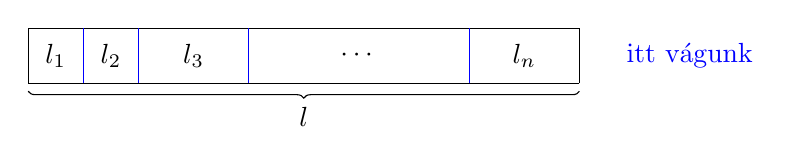
\begin{tikzpicture}[scale=0.7]
\draw (0,0) -- (10,0);
\draw (0,1) -- (10,1);

\draw (0,0) -- (0,1);
\draw[blue] (1,0) -- (1,1);
\draw[blue] (2,0) -- (2,1);
\draw[blue] (4,0) -- (4,1);
\draw[blue] (8,0) -- (8,1);
\draw (10,0) -- (10,1);

\node at (0.5,0.5) {$l_1$};
\node at (1.5,0.5) {$l_2$};
\node at (3,0.5) {$l_3$};
\node at (6,0.5) {$\cdots$};
\node at (9,0.5) {$l_n$};

\draw[decoration={mirror, brace, raise=0.1cm}, decorate] (0,0) -- (10,0);

\node at (5, -0.6) {$l$};
\node[blue] at (12, 0.5) {itt vágunk};
\end{tikzpicture}


Egy vágás úgy zajlik, hogy a már korábban "levágott" darabok valamelyikét felemeljük a vágóeszközre, és az ottani vágási pontok valamelyikén vágunk.
Egy ilyen vágás költsége legyen az épp vágott darab részeinek összege.

\textbf{Példa:}

\includegraphics[width=7cm]{gy/img/gy08_cut_step_1}\\
\textbf{1. vágás} (költség: 18)

\includegraphics[width=7cm]{gy/img/gy08_cut_step_2}\\
\textbf{2. vágás} (költség: 11)

\includegraphics[width=7cm]{gy/img/gy08_cut_step_3}\\
\textbf{3. vágás} (költség: 7)

\includegraphics[width=7cm]{gy/img/gy08_cut_step_4}\\
\textbf{4. vágás} (költség: 7)

\includegraphics[width=7cm]{gy/img/gy08_cut_step_5}\\
\textbf{5. vágás} (költség: 4)

\includegraphics[width=7cm]{gy/img/gy08_cut_step_6}\\
\textbf{6. vágás} (költség: 5)

\includegraphics[width=7cm]{gy/img/gy08_cut_step_7}

\textbf{Költség összesen:} 52

Van ennél kisebb összköltségű vágássorozat?
Mi a legkisebb összköltség?

Vegyük észre az analógiát az optimális zárójelezés feladattal!
Várhatóan DP egy alkalmas módszer lesz a megoldásra, analóg módon a zárójelezéshez.

(margó szélére: ha $n$ darabra vágunk, összesen $(n-1)!$ lehetőség van erre, persze ezek közül nem mind "lényegesen különböző")

Részproblémák \rightarrow "infixek optimális szétvágása"

\textbf{HF.} részletek kidolgozása

\textbf{Változat:} a vágási pontokat is nekünk kell meghatározni (persze $l = l_1 + l_2 + \cdots + l_n$ továbbra is).
A példát tekintve itt megengedett első vágásnak a bal szélről levágni egy 4 hosszú darabot.

Érdemes visszafelé elképzelni a vágássorozatot ("ragasztások sorozata").

Példánkban:
\nopagebreak

\includegraphics[width=8cm]{gy/img/gy08_cut_reverse}

Mohó heurisztika: mindig a két legrövidebb darabot ragasztjuk összeadjuk
Bizonyítani kell, hogy ezek a lokálisan optimális lépések elvezetnek a globális optimumhoz.

Nagyon hatékony $\rightarrow$ kupaccal $\mathcal{O}(n \log n)$ lépés (eredeti változat DP-vel $\rightarrow \mathcal{O}(n^3)$).

Nagyon hasonló ez az egész az információtömörítésnél megismert Huffman algoritmushoz (Huffman-kódhoz).

\subsubsection*{2. Optimális bináris keresőfa}
Általában bináris keresőfákat dinamikusan változó adathalmazokra alkalmazunk.
Itt most statikus lesz az adathalmaz ezzel szemben.
Itt ismert az adatelemek keresési gyakorisága is.
Olyan bináris keresőfa megépítése a cél az adatelemekből, ahol a keresési út hosszának várható értéke minimális.
\clearpage
\section{gyakorlat (2025. november 12.)}
\subsection{"Sztringológia"}

Karaktersorozatok hasonlósága
\begin{itemize}[label=$\rightarrow$]
    \item Levenshtein távolság (optimális szekvenciaillesztés)
    \item leghosszabb közös részsorozat (LKR)
\end{itemize}
Mindkét esetben DP\\
$X = (x_1, x_2, \cdots, x_m)$ és $Y = (y_1, y_2, \cdots, y_n)$ $\rightarrow \mathcal{O}(mn)$


\subsubsection*{Leghosszabb közös részsorozat (LKR, előadáson "vázlatosan" volt)}
\setulcolor{black}
\textbf{Optimális részstruktúra tulajdonság}

$X_i = (x_1, x_2, \cdots, x_i)$ és $Y_j = (y_1, y_2, \cdots, y_j)$ prefixek LKR-jének meghatározása van éppen terítéken.

Tfh. $X_i$ és $Y_j$ egy LKR-je $Z_h = (z_1, z_2, \cdots, z_h)$

Ekkor\\
\textbf{(A)} Ha $x_i = y_j$, akkor $z_h = x_i = y_j$ és $Z' = (z_1, z_2, \cdots, z_{h-1})$ egy LKR $X_{i-1}$-hez és $Y_{j-1}$-hez.
A másik két esetben $x_i \neq y_j$, így biztosan $z_h \neq x_i$ vagy $z_h \neq y_j$.\\
\textbf{(B)} Ha $z_h \neq x_i$, akkor $Z$ egy LKR $x_{i-1}$-hez és $Y_j$-hez.\\
\textbf{(C)} Ha $z_h \neq y_j$, akkor $Z$ egy LKR $X_i$-hez és $y_{j-1}$-hez.

\textbf{Bizonyítás}\\
\textbf{(A)} Itt két állítás van!
Kezdjük azzal, hogy $z_h = x_i = y_j$.
Indirekt tfh. ez nem igaz, vagyis $z_h \neq x_i, y_j$.

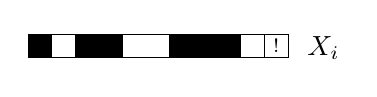
\begin{tikzpicture}[scale=0.3]
\draw(0,0) rectangle ++(11,1);
\draw[fill=black] (0,0) rectangle ++(1,1);
\draw[fill=black] (2,0) rectangle ++(1,1);
\draw[fill=black] (3,0) rectangle ++(1,1);
\draw[fill=black] (6,0) rectangle ++(1,1);
\draw[fill=black] (7,0) rectangle ++(1,1);
\draw[fill=black] (8,0) rectangle ++(1,1);
\draw (10,0) rectangle ++(1,1);
\node at (10.5, 0.5){\scriptsize !};

\node at (12.5, 0.4) {$X_i$};
\end{tikzpicture}

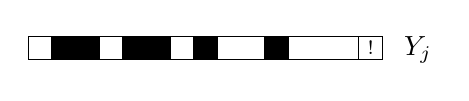
\begin{tikzpicture}[scale=0.3]
\draw(0,0) rectangle ++(15,1);
\draw[fill=black] (1,0) rectangle ++(1,1);
\draw[fill=black] (2,0) rectangle ++(1,1);
\draw[fill=black] (4,0) rectangle ++(1,1);
\draw[fill=black] (5,0) rectangle ++(1,1);
\draw[fill=black] (7,0) rectangle ++(1,1);
\draw[fill=black] (10,0) rectangle ++(1,1);
\draw (14,0) rectangle ++(1,1);
\node at (14.5, 0.5){\scriptsize !};

\node at (16.5, 0.4) {$Y_j$};
\end{tikzpicture}


\begin{tikzpicture}[scale=0.3]
\draw[fill=black] (0,0) rectangle ++(1,1);
\end{tikzpicture}
-k $\rightarrow Z$

Ám ekkor $Z$ biztos nem LKR $x_i$-hez és $Y_j$-hez, hiszen $Z$ végére írva az $x_i = y_j$ karaktert egy $Z$-nél hosszabb közös részsorozatát látjuk $X_i$-nek és $Y_j$-nek.

Ezek után jöjjön a második rész.
Most $Z'$ nyilván közös részsorozata $X_{i-1}$-nek és $Y_{j-1}$-nek.
Indirekt tfh. $Z'$ nem LKR $X_{i-1}$-hez és $Y_{j-1}$-hez, vagyis van olyan $Z'$-nél hosszabb $Z'$ sorozat, amely közös részsorozata $X_{i-1}$-nek és $Y_{j-1}$-nek.
Ha most $Z"$ végére írjuk az $x_i = y_j$ karaktert, az egy $Z$-nél hosszabb közös részsorozata lesz $X_i$-nek és $Y_j$-nek, \textbf{ellentmondás}.

\textbf{(B)} Most egyrészt $Z$ közös részsorozata $X_{i-1}$-nek és $Y_j$-nek, másrészt ha lenne egy $Z$-nél hosszabb közös részsorozata $X_{i-1}$-nek és $Y_j$-nek, az egy $Z$-nél hosszabb közös részsorozata lenne $X_i$-nek és $Y_j$-nek, ami nem lehet.

\textbf{(C)} analóg módon (B)-hez.

\textbf{Rekurzió}

$
l[i, j] = min
\begin{cases}
    0 & \text{ha $i=0$ vagy $j=0$}\\
    l[i-1, j-1] + 1 & \text{ha $i,j \geq 1$ és $x_i = y_j$}\\
    max \{l[i-1, j], l[i, j-1]\} & \text{ha $i,j \geq 1$ és $x_i \neq y_j$}\\
\end{cases}
$

\sethlcolor{orange}
\textbf{Példa} \hl{(zh. feladat)}:
\begin{flalign*}
    & X = (A, B, C, B, C, A, B, B, A, C) &&\\
    & Y = (B, A, A, C, B, B, A, A, C, B, C) &&
\end{flalign*}

\textbf{Kitöltés menete:}\\
Összehasonlítjuk a sorhoz és az oszlophoz tartozó két betűt.
\begin{itemize}
    \item Ha megegyeznek (rekurzív képlet 2. esete): az átlósan eggyel fentebb és vízszintesen előző elem + 1
    \item Ha különböznek (rekurzív képlet 3. esete): a sorban előtte lévő elem és az oszlopban felette lévő elem közül a maximális (ha egyenlőek akkor a fölötte lévő)
\end{itemize}

A nyilak mutatják, hogy az adott cellában lévő elemet honnan vettük.
Ezek mentén visszafele haladva meghatározható a LKR.
    
$l[i,j] =$
\begin{tabular}{cccccccccccccc}
                           &                         &                        & B                                        & A                                              & \fcolorbox{blue}{white}{A}                                       & C                                                                & \fcolorbox{blue}{white}{B}                                       & \fcolorbox{blue}{white}{B}                                       & A                                                                & A                                                                & \fcolorbox{blue}{white}{C}                                       & \fcolorbox{blue}{white}{B}                                       & \fcolorbox{blue}{white}{C}                                       \\
                           &                         & 0                      & 1                                        & 2                                              & 3                                                                & 4                                                                & 5                                                                & 6                                                                & 7                                                                & 8                                                                & 9                                                                & 10                                                               & 11                                                               \\ \cline{3-14} 
                           & \multicolumn{1}{c|}{0}  & \multicolumn{1}{c|}{0} & \multicolumn{1}{c|}{0}                   & \multicolumn{1}{c|}{\cellcolor[HTML]{34CDF9}0} & \multicolumn{1}{c|}{0}                                           & \multicolumn{1}{c|}{0}                                           & \multicolumn{1}{c|}{0}                                           & \multicolumn{1}{c|}{0}                                           & \multicolumn{1}{c|}{0}                                           & \multicolumn{1}{c|}{0}                                           & \multicolumn{1}{c|}{0}                                           & \multicolumn{1}{c|}{0}                                           & \multicolumn{1}{c|}{0}                                           \\ \cline{3-14} 
\fcolorbox{blue}{white}{A} & \multicolumn{1}{c|}{1}  & \multicolumn{1}{c|}{0} & \multicolumn{1}{c|}{\angledarrow{90} 0}  & \multicolumn{1}{c|}{\angledarrow{135} 1}       & \multicolumn{1}{c|}{\cellcolor[HTML]{34CDF9}\angledarrow{135} 1} & \multicolumn{1}{c|}{\cellcolor[HTML]{34CDF9}\angledarrow{180} 1} & \multicolumn{1}{c|}{\angledarrow{180} 1}                         & \multicolumn{1}{c|}{\angledarrow{180} 1}                         & \multicolumn{1}{c|}{\angledarrow{135} 1}                         & \multicolumn{1}{c|}{\angledarrow{135} 1}                                      & \multicolumn{1}{c|}{\angledarrow{180} 1}                         & \multicolumn{1}{c|}{\angledarrow{180} 1}                         & \multicolumn{1}{c|}{\angledarrow{180} 1}                         \\ \cline{3-14} 
\fcolorbox{blue}{white}{B} & \multicolumn{1}{c|}{2}  & \multicolumn{1}{c|}{0} & \multicolumn{1}{c|}{\angledarrow{135} 1} & \multicolumn{1}{c|}{\angledarrow{90} 1}        & \multicolumn{1}{c|}{\angledarrow{90} 1}                          & \multicolumn{1}{c|}{\angledarrow{90} 1}                          & \multicolumn{1}{c|}{\cellcolor[HTML]{34CDF9}\angledarrow{135} 2} & \multicolumn{1}{c|}{\angledarrow{135} 2}                         & \multicolumn{1}{c|}{\angledarrow{180} 2}                         & \multicolumn{1}{c|}{\angledarrow{180} 2}                         & \multicolumn{1}{c|}{\angledarrow{180} 2}                         & \multicolumn{1}{c|}{\angledarrow{135} 2}                         & \multicolumn{1}{c|}{\angledarrow{180} 2}                         \\ \cline{3-14} 
C                          & \multicolumn{1}{c|}{3}  & \multicolumn{1}{c|}{0} & \multicolumn{1}{c|}{\angledarrow{90} 1}  & \multicolumn{1}{c|}{\angledarrow{90} 1}        & \multicolumn{1}{c|}{\angledarrow{90} 1}                          & \multicolumn{1}{c|}{\angledarrow{135} 2}                         & \multicolumn{1}{c|}{\cellcolor[HTML]{34CDF9}\angledarrow{90} 2}  & \multicolumn{1}{c|}{\angledarrow{90} 2}                          & \multicolumn{1}{c|}{\angledarrow{90} 2}                          & \multicolumn{1}{c|}{\angledarrow{90} 2}                          & \multicolumn{1}{c|}{\angledarrow{135} 3}                         & \multicolumn{1}{c|}{\angledarrow{180} 3}                         & \multicolumn{1}{c|}{\angledarrow{135} 3}                         \\ \cline{3-14} 
\fcolorbox{blue}{white}{B} & \multicolumn{1}{c|}{4}  & \multicolumn{1}{c|}{0} & \multicolumn{1}{c|}{\angledarrow{135} 1} & \multicolumn{1}{c|}{\angledarrow{90} 1}        & \multicolumn{1}{c|}{\angledarrow{90} 1}                          & \multicolumn{1}{c|}{\angledarrow{90} 2}                          & \multicolumn{1}{c|}{\angledarrow{135} 3}                         & \multicolumn{1}{c|}{\cellcolor[HTML]{34CDF9}\angledarrow{135} 3} & \multicolumn{1}{c|}{\cellcolor[HTML]{34CDF9}\angledarrow{180} 3} & \multicolumn{1}{c|}{\cellcolor[HTML]{34CDF9}\angledarrow{180} 3} & \multicolumn{1}{c|}{\angledarrow{90} 3}                          & \multicolumn{1}{c|}{\angledarrow{135} 4}                         & \multicolumn{1}{c|}{\angledarrow{180} 4}                         \\ \cline{3-14} 
\fcolorbox{blue}{white}{C} & \multicolumn{1}{c|}{5}  & \multicolumn{1}{c|}{0} & \multicolumn{1}{c|}{\angledarrow{90} 1}  & \multicolumn{1}{c|}{\angledarrow{90} 1}        & \multicolumn{1}{c|}{\angledarrow{90} 1}                          & \multicolumn{1}{c|}{\angledarrow{135} 2}                         & \multicolumn{1}{c|}{\angledarrow{90} 3}                          & \multicolumn{1}{c|}{\angledarrow{90} 3}                          & \multicolumn{1}{c|}{\angledarrow{90} 3}                          & \multicolumn{1}{c|}{\angledarrow{90} 3}                          & \multicolumn{1}{c|}{\cellcolor[HTML]{34CDF9}\angledarrow{135} 4} & \multicolumn{1}{c|}{\angledarrow{90} 4}                          & \multicolumn{1}{c|}{\angledarrow{135} 5}                         \\ \cline{3-14} 
A                          & \multicolumn{1}{c|}{6}  & \multicolumn{1}{c|}{0} & \multicolumn{1}{c|}{\angledarrow{90} 1}  & \multicolumn{1}{c|}{\angledarrow{135} 2}       & \multicolumn{1}{c|}{\angledarrow{135} 2}                         & \multicolumn{1}{c|}{\angledarrow{90} 2}                          & \multicolumn{1}{c|}{\angledarrow{90} 3}                          & \multicolumn{1}{c|}{\angledarrow{90} 3}                          & \multicolumn{1}{c|}{\angledarrow{135} 4}                         & \multicolumn{1}{c|}{\angledarrow{135} 4}                         & \multicolumn{1}{c|}{\cellcolor[HTML]{34CDF9}\angledarrow{90} 4}  & \multicolumn{1}{c|}{\angledarrow{90} 4}                          & \multicolumn{1}{c|}{\angledarrow{90} 5}                          \\ \cline{3-14} 
B                          & \multicolumn{1}{c|}{7}  & \multicolumn{1}{c|}{0} & \multicolumn{1}{c|}{\angledarrow{135} 1} & \multicolumn{1}{c|}{\angledarrow{90} 2}        & \multicolumn{1}{c|}{\angledarrow{90} 2}                          & \multicolumn{1}{c|}{\angledarrow{90} 2}                          & \multicolumn{1}{c|}{\angledarrow{135} 3}                         & \multicolumn{1}{c|}{\angledarrow{135} 4}                         & \multicolumn{1}{c|}{\angledarrow{90} 4}                          & \multicolumn{1}{c|}{\angledarrow{90} 4}                          & \multicolumn{1}{c|}{\cellcolor[HTML]{34CDF9}\angledarrow{90} 4}  & \multicolumn{1}{c|}{\angledarrow{135} 5}                         & \multicolumn{1}{c|}{\angledarrow{90} 5}                          \\ \cline{3-14} 
\fcolorbox{blue}{white}{B} & \multicolumn{1}{c|}{8}  & \multicolumn{1}{c|}{0} & \multicolumn{1}{c|}{\angledarrow{135} 1} & \multicolumn{1}{c|}{\angledarrow{90} 2}        & \multicolumn{1}{c|}{\angledarrow{90} 2}                          & \multicolumn{1}{c|}{\angledarrow{90} 2}                          & \multicolumn{1}{c|}{\angledarrow{135} 3}                         & \multicolumn{1}{c|}{\angledarrow{135} 4}                         & \multicolumn{1}{c|}{\angledarrow{90} 4}                          & \multicolumn{1}{c|}{\angledarrow{90} 4}                          & \multicolumn{1}{c|}{\angledarrow{90} 4}                          & \multicolumn{1}{c|}{\cellcolor[HTML]{34CDF9}\angledarrow{135} 5} & \multicolumn{1}{c|}{\angledarrow{90} 5}                          \\ \cline{3-14} 
A                          & \multicolumn{1}{c|}{9}  & \multicolumn{1}{c|}{0} & \multicolumn{1}{c|}{\angledarrow{90} 1}  & \multicolumn{1}{c|}{\angledarrow{135} 2}       & \multicolumn{1}{c|}{\angledarrow{135} 3}                         & \multicolumn{1}{c|}{\angledarrow{180} 3}                         & \multicolumn{1}{c|}{\angledarrow{90} 3}                          & \multicolumn{1}{c|}{\angledarrow{90} 4}                          & \multicolumn{1}{c|}{\angledarrow{135} 5}                         & \multicolumn{1}{c|}{\angledarrow{135} 5}                         & \multicolumn{1}{c|}{\angledarrow{180} 5}                         & \multicolumn{1}{c|}{\cellcolor[HTML]{34CDF9}\angledarrow{90} 5}  & \multicolumn{1}{c|}{\angledarrow{90} 5}                          \\ \cline{3-14} 
\fcolorbox{blue}{white}{C} & \multicolumn{1}{c|}{10} & \multicolumn{1}{c|}{0} & \multicolumn{1}{c|}{\angledarrow{90} 1}  & \multicolumn{1}{c|}{\angledarrow{90} 2}        & \multicolumn{1}{c|}{\angledarrow{90} 3}                          & \multicolumn{1}{c|}{\angledarrow{135} 4}                         & \multicolumn{1}{c|}{\angledarrow{180} 4}                         & \multicolumn{1}{c|}{\angledarrow{90} 4}                          & \multicolumn{1}{c|}{\angledarrow{90} 5}                          & \multicolumn{1}{c|}{\angledarrow{90} 5}                          & \multicolumn{1}{c|}{\angledarrow{135} 6}                         & \multicolumn{1}{c|}{\angledarrow{180} 6}                         & \multicolumn{1}{c|}{\cellcolor[HTML]{34CDF9}\angledarrow{135} 6} \\ \cline{3-14} 
\end{tabular}

\textbf{LKR hossz:} 6\\
\textbf{LKR:} {\color{blue} ABBCBC} (van más is!)\\
Az előbbi $X$ és $Y$ Levenshtein távolsága.

Itt még kell valami:
\begin{flalign*}
    & g = 3 &&\\
    & c["p", "q"] = 5 \text{ (a csere 5 költségű)} &&\\
    & c["p", "p"] = 0 \text{ (a nem-csere 0 költségű)} &&
\end{flalign*}
\clearpage
\section{gyakorlat (2025. november 19.)}
\subsection{}
\clearpage
\section{gyakorlat (2025. november 19.)}
\subsection{Hátizsák feladat}
\sethlcolor{orange}
\textbf{Példa} \hl{(zh. feladat)}:\\
\begin{tabular}{c|c|c|c|c|c|c|c|}
\cline{2-8}
i     & 1  & 2  & 3  & 4  & 5 & 6  & 7  \\ \cline{2-8} 
$w_i$ & 4  & 5  & 3  & 1  & 1 & 4  & 3  \\ \cline{2-8} 
$v_i$ & 40 & 60 & 10 & 10 & 3 & 20 & 60 \\ \cline{2-8} 
\end{tabular}

$W = 10$ (hátizsák kapacitása)

Részfeladatok: az első néhány tárggyal kell megtölteni optimálisan kisebb hátizsákokat.

Kitöltés menete:\\
Az oszlop a hátizsák kapacitása, a sor a hátizsákba rakott érték.
Minden sorhoz tartozik egy tárgy (az $i.$ sorhoz $t_i$ és $v_i$) egy \sethlcolor{red}\hl{súly}/\sethlcolor{yellow}\hl{érték} párral.
Megnézzük milyen \sethlcolor{lime}\hl{érték} van a jelenlegi cellától eggyel fentebbi cellában.
Visszalépünk abban a sorban \sethlcolor{red}\hl{súly} cellát.
Amelyik cellához \sethlcolor{pink}\hl{jutottunk}, azt hozzáadjuk az \sethlcolor{yellow}\hl{értékhez}.
Az összeg és a cella feletti \sethlcolor{lime}\hl{érték} közül a nagyobb lesz a cella tartalma.

Előadásról:
$
h[i, j] = max
\begin{cases}
    v_i + h[i-1, j-w_i]\\
    h[i-1, j]\\
\end{cases}
$

Ha pl. az sorhoz tartozó tárgy súlya 4, akkor a 0, 1, 2, 3 indexű oszlopok csak másolódnak, mert nem tudunk 4-et visszalépni a felette lévő sorban.
Azaz, 0, 1, 2, 3 kapacitású hátizsákba nem fér bele a 4 súlyú tárgy.
Minden sorban azt nézzük, hogy a sorhoz tartozó tárgyat érdemes-e belerakni a hátizsákba.

\sethlcolor{yellow}
\begin{tabular}{ccccccccccccc}
     & i\textbackslash{}j                             & 0                                              & 1                       & 2                       & 3                       & 4                       & 5                                               & 6                                               & 7                                               & 8                        & 9                              & 10                                               \\ \cline{3-13} 
     & \multicolumn{1}{c|}{0}                         & \multicolumn{1}{c|}{0}                         & \multicolumn{1}{c|}{0}  & \multicolumn{1}{c|}{0}  & \multicolumn{1}{c|}{0}  & \multicolumn{1}{c|}{0}  & \multicolumn{1}{c|}{0}                          & \multicolumn{1}{c|}{0}                          & \multicolumn{1}{c|}{0}                          & \multicolumn{1}{c|}{0}   & \multicolumn{1}{c|}{0}         & \multicolumn{1}{c|}{0}                           \\ \cline{3-13} 
4/40 & \multicolumn{1}{c|}{1}                         & \multicolumn{1}{c|}{\cellcolor[HTML]{34CDF9}0} & \multicolumn{1}{c|}{0}  & \multicolumn{1}{c|}{0}  & \multicolumn{1}{c|}{0}  & \multicolumn{1}{c|}{\sethlcolor{pink}\hl{40}} & \multicolumn{1}{c|}{40}                         & \multicolumn{1}{c|}{40}                         & \multicolumn{1}{c|}{40}                         & \multicolumn{1}{c|}{40}  & \multicolumn{1}{c|}{\sethlcolor{lime}\hl{40}}        & \multicolumn{1}{c|}{40}                          \\ \cline{3-13} 
\sethlcolor{red}\hl{5}/\sethlcolor{yellow}\hl{60} & \multicolumn{1}{c|}{\fcolorbox{blue}{white}{2}} & \multicolumn{1}{c|}{0}                         & \multicolumn{1}{c|}{0}  & \multicolumn{1}{c|}{0}  & \multicolumn{1}{c|}{0}  & \multicolumn{1}{c|}{40} & \multicolumn{1}{c|}{\cellcolor[HTML]{34CDF9}60} & \multicolumn{1}{c|}{60}                         & \multicolumn{1}{c|}{60}                         & \multicolumn{1}{c|}{60}  & \multicolumn{1}{c|}{max(\sethlcolor{lime}\hl{40}, (\sethlcolor{pink}\hl{40}+\sethlcolor{yellow}\hl{60}))=100} & \multicolumn{1}{c|}{100}                         \\ \cline{3-13} 
3/10 & \multicolumn{1}{c|}{3}                         & \multicolumn{1}{c|}{0}                         & \multicolumn{1}{c|}{0}  & \multicolumn{1}{c|}{0}  & \multicolumn{1}{c|}{10} & \multicolumn{1}{c|}{40} & \multicolumn{1}{c|}{\cellcolor[HTML]{34CDF9}60} & \multicolumn{1}{c|}{60}                         & \multicolumn{1}{c|}{60}                         & \multicolumn{1}{c|}{70}  & \multicolumn{1}{c|}{100}       & \multicolumn{1}{c|}{100}                         \\ \cline{3-13} 
1/10 & \multicolumn{1}{c|}{\fcolorbox{blue}{white}{4}} & \multicolumn{1}{c|}{0}                         & \multicolumn{1}{c|}{10} & \multicolumn{1}{c|}{10} & \multicolumn{1}{c|}{10} & \multicolumn{1}{c|}{40} & \multicolumn{1}{c|}{60}                         & \multicolumn{1}{c|}{\cellcolor[HTML]{34CDF9}70} & \multicolumn{1}{c|}{70}                         & \multicolumn{1}{c|}{70}  & \multicolumn{1}{c|}{100}       & \multicolumn{1}{c|}{110}                         \\ \cline{3-13} 
1/3  & \multicolumn{1}{c|}{\fcolorbox{blue}{white}{5}} & \multicolumn{1}{c|}{0}                         & \multicolumn{1}{c|}{10} & \multicolumn{1}{c|}{13} & \multicolumn{1}{c|}{13} & \multicolumn{1}{c|}{40} & \multicolumn{1}{c|}{60}                         & \multicolumn{1}{c|}{70}                         & \multicolumn{1}{c|}{\cellcolor[HTML]{34CDF9}73} & \multicolumn{1}{c|}{73}  & \multicolumn{1}{c|}{100}       & \multicolumn{1}{c|}{110}                         \\ \cline{3-13} 
4/20 & \multicolumn{1}{c|}{6}                         & \multicolumn{1}{c|}{0}                         & \multicolumn{1}{c|}{10} & \multicolumn{1}{c|}{13} & \multicolumn{1}{c|}{13} & \multicolumn{1}{c|}{40} & \multicolumn{1}{c|}{60}                         & \multicolumn{1}{c|}{70}                         & \multicolumn{1}{c|}{\cellcolor[HTML]{34CDF9}73} & \multicolumn{1}{c|}{73}  & \multicolumn{1}{c|}{100}       & \multicolumn{1}{c|}{110}                         \\ \cline{3-13} 
3/60 & \multicolumn{1}{c|}{\fcolorbox{blue}{white}{7}} & \multicolumn{1}{c|}{0}                         & \multicolumn{1}{c|}{10} & \multicolumn{1}{c|}{13} & \multicolumn{1}{c|}{60} & \multicolumn{1}{c|}{70} & \multicolumn{1}{c|}{73}                         & \multicolumn{1}{c|}{73}                         & \multicolumn{1}{c|}{100}                        & \multicolumn{1}{c|}{120} & \multicolumn{1}{c|}{130}       & \multicolumn{1}{c|}{\cellcolor[HTML]{34CDF9}133} \\ \cline{3-13} 
\end{tabular}

Eredmény leolvasása:\\
A jobb alsó sarokból indulunk szokás szerint.
A 7. sorban még nőtt az érték, tehát a 7. tárgyra szükség van, ezt "beragasztjuk" a hátizsákba.
Ekkor már beragaszottunk 3 kapacitásnyi tárgyat a 10 kapacitású hátizsákba.
Az első 7 kapacitást kell még valahogy kitölteni.
Ezért nézzük a 7. oszlopot és felfelé haladva a következő sort.
Ez a cella az előző sorhoz képest nem javult, azaz a 6. tárgyra nincs szükség.
Megyünk megint egy sorral fentebb, ugyanabban az oszlopban.
Ez javított az őt megelőző sorhoz képest, ezért erre a tárgyra szükség van.
Ezt ismételjük tovább.

Optimális megoldás: $t_2, t_4, t_5, t_7$
\clearpage
\include{gy/gy12}
\clearpage
\include{gy/gy13}
\end{document}